% ============================================================================
% AgroConecta — PIM IV
% Compilar com: pdflatex -interaction=nonstopmode pim.tex (duas vezes)
% ============================================================================
\documentclass[12pt,a4paper]{article}

% ============================================================================
% Estilo ABNT para o PIM IV — AgroConecta
% Baseado nas regras do manual do PIM (docs/manual.md) e na NBR 14724:2011.
% ============================================================================

% ---------------------------------------------------------------- página ----
\usepackage[a4paper,top=3cm,bottom=2cm,left=3cm,right=2cm]{geometry}

% ------------------------------------------------------------------ fontes ---
\usepackage[T1]{fontenc}
\usepackage[utf8]{inputenc}
\usepackage[portuguese]{babel}
\usepackage{helvet}
\renewcommand{\familydefault}{\sfdefault}

% ------------------------------------------------------------- espaçamento ---
\usepackage{setspace}
\onehalfspacing
\setlength{\parindent}{1.5cm}
\usepackage{indentfirst}
\setlength{\emergencystretch}{1.5em}

% --------------------------------------------------------------- títulos -----
\usepackage{titlesec}
\titleformat{\section}
  {\normalfont\bfseries\fontsize{12}{18}\selectfont}
  {\thesection}{0.8em}{}
\titlespacing*{\section}{0pt}{1.1\baselineskip}{0.7\baselineskip}

\titleformat{\subsection}
  {\normalfont\bfseries\fontsize{12}{18}\selectfont}
  {\thesubsection}{0.8em}{}
\titlespacing*{\subsection}{0pt}{0.9\baselineskip}{0.4\baselineskip}

\titleformat{\subsubsection}
  {\normalfont\itshape\fontsize{12}{18}\selectfont}
  {\thesubsubsection}{0.8em}{}
\titlespacing*{\subsubsection}{0pt}{0.8\baselineskip}{0.3\baselineskip}

% --------------------------------------------------------------- sumário -----
\usepackage{tocloft}
\addto\captionsportuguese{\renewcommand{\contentsname}{SUMÁRIO}}
\renewcommand{\cfttoctitlefont}{\hfill\bfseries\fontsize{12}{18}\selectfont}
\renewcommand{\cftaftertoctitle}{\hfill}
\renewcommand{\cftsecfont}{\normalfont}
\renewcommand{\cftsecpagefont}{\normalfont\bfseries}
\renewcommand{\cftsubsecfont}{\normalfont}
\renewcommand{\cftsubsecpagefont}{\normalfont}
\renewcommand{\cftsecleader}{\cftdotfill{\cftdotsep}}
\setlength{\cftsecindent}{0pt}
\setlength{\cftsubsecindent}{0pt}
\setlength{\cftsubsubsecindent}{0pt}
\setlength{\cftbeforesecskip}{0.4\baselineskip}

% ---------------------------------------------------------------- figuras ----
\usepackage{graphicx}
\usepackage{float}
\usepackage{needspace}
\usepackage{caption}
\captionsetup{
  position=above,
  labelfont=bf,
  labelsep=endash,
  justification=centering,
  singlelinecheck=false,
  font=small,
  skip=6pt
}
\renewcommand{\figurename}{Figura}
\renewcommand{\tablename}{Tabela}

% Fonte de figura/tabela, em 10 pt, logo abaixo do elemento.
\newcommand{\fonte}[1]{%
  \par\vspace{2pt}%
  {\fontsize{10}{12}\selectfont\itshape Fonte: #1\par}%
}

% Atalho: figura com legenda e fonte.
% #1 arquivo, #2 legenda, #3 fonte
\newcommand{\figura}[3]{%
  \begin{figure}[H]
    \centering
    \caption{#2}
    \includegraphics[width=0.92\textwidth]{#1}
    \fonte{#3}
  \end{figure}
}

% Atalho para tabela simples (uma coluna de texto corrida).
% ------------------------------------------------------------- citações ------
% Citação longa: 4 cm da margem esquerda, corpo 10, espaço simples.
\newenvironment{citacao}
  {\begin{spacing}{1}\begin{list}{}{%
     \setlength{\leftmargin}{4cm}\setlength{\rightmargin}{0pt}%
     \setlength{\listparindent}{0pt}\setlength{\itemindent}{0pt}%
     \setlength{\topsep}{0.5\baselineskip}\setlength{\parsep}{0pt}}%
   \item[]\fontsize{10}{12}\selectfont}
  {\end{list}\end{spacing}}

% ------------------------------------------------------------- listas --------
\usepackage{enumitem}
\setlist[itemize]{leftmargin=1.5cm,topsep=0.3\baselineskip,itemsep=0.15\baselineskip}
\setlist[enumerate]{leftmargin=1.5cm,topsep=0.3\baselineskip,itemsep=0.15\baselineskip}

% --------------------------------------------------------------- diagramas ---
\usepackage{tikz}
\usetikzlibrary{positioning, arrows.meta, shapes.geometric, calc, fit, backgrounds}

% --------------------------------------------------------------- tabelas -----
\usepackage{booktabs}
\usepackage{array}
\newcolumntype{L}[1]{>{\raggedright\arraybackslash}p{#1}}
\usepackage{longtable}
\usepackage{multirow}
\setlength{\tabcolsep}{4pt}

% --------------------------------------------------------------- código ------
\usepackage{xcolor}
\usepackage{listings}
\lstdefinestyle{abnt}{
  basicstyle=\ttfamily\fontsize{8}{9.5}\selectfont,
  breaklines=true,
  columns=fullflexible,
  keepspaces=true,
  showstringspaces=false,
  frame=none,
  aboveskip=1.2\baselineskip,
  belowskip=0.8\baselineskip,
  extendedchars=true,
  inputencoding=utf8,
  literate=
    {á}{{\'a}}1 {à}{{\`a}}1 {â}{{\^a}}1 {ã}{{\~a}}1 {ä}{{\"a}}1
    {Á}{{\'A}}1 {À}{{\`A}}1 {Â}{{\^A}}1 {Ã}{{\~A}}1
    {é}{{\'e}}1 {ê}{{\^e}}1 {É}{{\'E}}1 {Ê}{{\^E}}1
    {í}{{\'i}}1 {î}{{\^i}}1 {Í}{{\'I}}1
    {ó}{{\'o}}1 {ô}{{\^o}}1 {õ}{{\~o}}1 {Ó}{{\'O}}1 {Ô}{{\^O}}1 {Õ}{{\~O}}1
    {ú}{{\'u}}1 {ü}{{\"u}}1 {Ú}{{\'U}}1 {Ü}{{\"U}}1
    {ç}{{\c c}}1 {Ç}{{\c C}}1
    {“}{{"}}1 {”}{{"}}1 {‘}{{`}}1 {’}{{'}}1
    {–}{{--}}1 {—}{{---}}1
}
\lstset{style=abnt}

% --------------------------------------------------------------- cabeçalho ---
\usepackage{fancyhdr}
\fancypagestyle{abnt}{%
  \fancyhf{}%
  \fancyhead[R]{\fontsize{10}{12}\selectfont\thepage}%
  \renewcommand{\headrulewidth}{0pt}%
  \renewcommand{\footrulewidth}{0pt}%
}
\fancypagestyle{vazio}{%
  \fancyhf{}%
  \renewcommand{\headrulewidth}{0pt}%
  \renewcommand{\footrulewidth}{0pt}%
}
\fancypagestyle{plain}{%
  \fancyhf{}%
  \renewcommand{\headrulewidth}{0pt}%
  \renewcommand{\footrulewidth}{0pt}%
}

% --------------------------------------------------------------- hyperlinks --
\usepackage[hidelinks,unicode]{hyperref}
\usepackage{xurl}
\hypersetup{
  pdftitle={AgroConecta: plataforma corporativa integrada para gestão da cadeia de suprimentos e inclusão digital na agricultura familiar},
  pdfauthor={[NOME]},
  pdfsubject={Projeto Integrado Multidisciplinar IV}
}

% ------------------------------------------------------- hifenização ---------
\hyphenation{AgroConecta}

% ------------------------------------------------------- comandos auxiliares --
% Título de elemento pré-textual (centralizado, maiúsculo, negrito).
\newcommand{\titulopretextual}[1]{%
  \begin{center}
    \bfseries\fontsize{12}{18}\selectfont #1
  \end{center}
  \vspace{0.5\baselineskip}
}

% Entrada de referência: sem recuo, espaço simples, separada por uma linha.
\newcommand{\refbib}[1]{%
  \par\begingroup
  \setlength{\parindent}{0pt}%
  \setlength{\parskip}{0pt}%
  \noindent #1\par
  \vspace{0.75\baselineskip}%
  \endgroup
}


\begin{document}

% ============================================================================
% Elementos pré-textuais: capa, folha de rosto, resumo, abstract e sumário
% ============================================================================

% ------------------------------------------------------------------- CAPA ----
\begin{titlepage}
  \begin{center}
    \fontsize{12}{18}\selectfont
    \textbf{UNIVERSIDADE PAULISTA -- UNIP}\\[0.2\baselineskip]
    Projeto Integrado Multidisciplinar\\[0.2\baselineskip]
    Curso Superior de Tecnologia em\\ Análise e Desenvolvimento de Sistemas

    \vspace{2.2cm}

    \textbf{[NOME DO ALUNO] -- [RA]}\\[0.25\baselineskip]
    \textbf{[NOME DO ALUNO] -- [RA]}

    \vspace{2.4cm}

    {\fontsize{14}{21}\selectfont\bfseries
      AGROCONECTA: PLATAFORMA CORPORATIVA INTEGRADA PARA GESTÃO DA CADEIA
      DE SUPRIMENTOS E INCLUSÃO DIGITAL NA AGRICULTURA FAMILIAR\par}

    \vfill

    São Paulo -- SP\\
    2026
  \end{center}
\end{titlepage}

% --------------------------------------------------------- FOLHA DE ROSTO ---
\begin{titlepage}
  \begin{center}
    \fontsize{12}{18}\selectfont
    \textbf{[NOME DO ALUNO] -- [RA]}\\[0.25\baselineskip]
    \textbf{[NOME DO ALUNO] -- [RA]}

    \vspace{2.6cm}

    {\fontsize{14}{21}\selectfont\bfseries
      AGROCONECTA: PLATAFORMA CORPORATIVA INTEGRADA PARA GESTÃO DA CADEIA
      DE SUPRIMENTOS E INCLUSÃO DIGITAL NA AGRICULTURA FAMILIAR\par}

    \vspace{2.5cm}
  \end{center}

  \noindent\hspace*{5.5cm}%
  \begin{minipage}{9.5cm}
    \raggedright
    \fontsize{11}{16}\selectfont
    Projeto Integrado Multidisciplinar apresentado à Universidade Paulista --
    UNIP, como requisito parcial para a obtenção do título de tecnólogo em
    Análise e Desenvolvimento de Sistemas.

    \vspace{0.6\baselineskip}
    Orientador(a): [NOME DO ORIENTADOR]
  \end{minipage}

  \vfill
  \begin{center}
    \fontsize{12}{18}\selectfont
    São Paulo -- SP\\
    2026
  \end{center}
\end{titlepage}

% ----------------------------------------------------------------- RESUMO ----
\setcounter{page}{3}
\pagestyle{vazio}
\begingroup
\setstretch{1}
\titulopretextual{RESUMO}

A transformação digital de cadeias produtivas agroalimentares exige soluções que
conectem planejamento de negócio, aplicações corporativas, banco de dados,
infraestrutura e gestão ágil em um único ecossistema. Este trabalho apresenta o
AgroConecta, plataforma corporativa integrada para a gestão da cadeia de
suprimentos e a inclusão digital da agricultura familiar. O problema identificado
é a assimetria de informação entre cooperativas, produtores familiares,
compradores institucionais e transportadores, que provoca perdas de produção,
fragilidade na rastreabilidade e baixa capacidade de escoamento. A metodologia
adotou pesquisa aplicada de natureza qualitativa, apoiada em levantamento
documental, modelagem de negócio e desenvolvimento incremental com práticas ágeis
(Scrum e Kanban). A solução foi construída sobre uma arquitetura em camadas com
.NET 10 e ASP.NET Core, oferecendo aplicação Web com autenticação por cookie e
API REST protegida por JWT, além de um aplicativo mobile em React Native e Expo
com operação offline. O banco de dados relacional em SQL Server 2022 contempla
quatorze tabelas de negócio, três procedimentos armazenados e três gatilhos de
auditoria e movimentação de estoque, validados por scripts completos. Os
resultados incluem um fluxo ponta a ponta de produto, lote, pedido, rota, entrega
com evidência fotográfica e geolocalização, e faturamento, com 159 testes
automatizados aprovados e cobertura superior a 90\% nas camadas de domínio e
aplicação. Conclui-se que a plataforma atende aos requisitos técnicos e
organizacionais do projeto, amplia a transparência da cadeia e cria condições
concretas de inclusão produtiva para agricultores familiares.

\vspace{0.5\baselineskip}
\noindent\textbf{Palavras-chave:} Agricultura familiar. Transformação digital.
Plataforma corporativa. Desenvolvimento Web. Aplicativo mobile. Banco de dados.
\endgroup

% ---------------------------------------------------------------- ABSTRACT ---
\newpage
\begingroup
\setstretch{1}
\begin{otherlanguage}{english}
\titulopretextual{ABSTRACT}

The digital transformation of agrifood supply chains requires solutions that
connect business planning, corporate applications, databases, infrastructure and
agile management in a single ecosystem. This paper presents AgroConecta, an
integrated corporate platform for supply chain management and digital inclusion
of family farming. The identified problem is the information asymmetry among
cooperatives, family producers, institutional buyers and transporters, which
causes production losses, weak traceability and low market access. The
methodology adopted applied qualitative research supported by document analysis,
business modeling and incremental development with agile practices (Scrum and
Kanban). The solution was built on a layered architecture with .NET 10 and
ASP.NET Core, providing a Web application with cookie authentication and a REST
API protected by JWT, as well as a React Native and Expo mobile application with
offline operation. The relational database on SQL Server 2022 comprises fourteen
business tables, three stored procedures and three triggers for auditing and
inventory movement, validated by complete scripts. The results include an
end-to-end flow of product, harvest lot, order, route, delivery with photographic
and geolocation evidence, and invoicing, with 159 automated tests passing and
coverage above 90\% in the domain and application layers. It is concluded that
the platform meets the technical and organizational requirements of the project,
increases supply chain transparency and creates concrete conditions for
productive inclusion of family farmers.

\vspace{0.5\baselineskip}
\noindent\textbf{Keywords:} Family farming. Digital transformation. Corporate
platform. Web development. Mobile application. Database.
\end{otherlanguage}
\endgroup

% ---------------------------------------------------------------- SUMÁRIO ----
\newpage
\begingroup
\setstretch{1}
\tableofcontents
\endgroup


% ============================================================== INTRODUÇÃO ===
\newpage
\pagestyle{abnt}
\section*{INTRODUÇÃO}
\addcontentsline{toc}{section}{INTRODUÇÃO}

A transformação digital deixou de ser um diferencial competitivo para se tornar
condição de sobrevivência em cadeias produtivas intensivas em informação. No
agronegócio, esse movimento é particularmente sensível porque envolve agentes com
níveis muito distintos de maturidade tecnológica: de um lado, compradores
institucionais, distribuidores e cooperativas que operam sistemas integrados de
gestão; de outro, agricultores familiares que, muitas vezes, registram a produção
em cadernos e negociam preços por telefone. A assimetria entre esses dois mundos
gera perdas de produção, dificulta a rastreabilidade sanitária e reduz a renda de
quem está na base da cadeia.

A agricultura familiar responde por parcela expressiva dos estabelecimentos
rurais brasileiros e por parte relevante da produção de alimentos que chega à
mesa da população (IBGE, 2019). Apesar dessa importância, o segmento enfrenta
dificuldades estruturais de acesso a mercados, crédito, assistência técnica e
informação de preços. Programas de compras públicas, como o Programa Nacional de
Alimentação Escolar (PNAE) e o Programa de Aquisição de Alimentos (PAA),
ampliaram o espaço institucional para esses produtores, mas criaram também novas
exigências operacionais: emissão de documentos, comprovação de entrega,
rastreabilidade de lotes e prestação de contas. Sem ferramentas adequadas, tais
exigências acabam funcionando como barreiras adicionais.

Este trabalho parte de uma organização fictícia, a \textbf{Cooperativa
Agropecuária Vale Verde}, sediada na região de Campinas (SP), que reúne
produtores familiares de diferentes comunidades -- tradicionais, quilombolas,
assentados e indígenas -- e comercializa hortifrúti, grãos e produtos
beneficiados para escolas, restaurantes universitários e redes varejistas. A
cooperativa cresceu sem que seus controles evoluíssem na mesma proporção: os
pedidos chegam por canais variados, a programação de rotas é feita em planilhas
e a comprovação de entrega depende de fotografias enviadas por aplicativo de
mensagens, sem vínculo com o pedido ou com a nota fiscal.

Diante desse cenário, o objetivo geral deste Projeto Integrado Multidisciplinar
é desenvolver uma solução tecnológica corporativa integrada que apoie a
transformação digital da cooperativa, cobrindo desde o planejamento do negócio e
o desenvolvimento das aplicações Web e mobile até a modelagem do banco de dados,
a definição da infraestrutura em nuvem e o gerenciamento ágil do projeto. Os
objetivos específicos são: caracterizar a organização e seus processos;
estruturar a proposta de valor e a viabilidade da solução; incorporar práticas de
inclusão digital, acessibilidade e proteção de dados; implementar uma aplicação
Web administrativa e uma API REST segura; desenvolver um aplicativo mobile com
operação offline para produtores e motoristas; projetar o banco de dados
relacional com procedimentos armazenados e gatilhos; planejar a implantação em
nuvem com pipeline de integração e entrega contínuas; e organizar o trabalho com
Product Backlog, Sprint Backlog e quadro Kanban.

A metodologia adotada caracteriza-se como pesquisa aplicada de abordagem
qualitativa, com objetivo exploratório e descritivo. O procedimento técnico
combinou levantamento documental sobre o domínio agroalimentar, modelagem de
negócio e desenvolvimento incremental de software. O ciclo de vida seguiu
práticas ágeis: requisitos priorizados em Product Backlog, entregas em quatro
sprints de duas semanas, revisões ao final de cada incremento e uso de quadro
Kanban para visualizar o fluxo de trabalho. A engenharia utilizou arquitetura em
camadas (domínio, aplicação, infraestrutura e apresentação), contrato OpenAPI
como fonte de verdade para o consumo das APIs e automação de testes em todos os
níveis. O projeto foi conduzido em duas frentes paralelas -- núcleo
corporativo/Web e aplicativo mobile -- integradas continuamente à linha principal
do repositório.

Quanto à estrutura, além desta introdução, o trabalho apresenta nove capítulos
que correspondem às etapas solicitadas no manual do PIM IV. O primeiro
caracteriza a organização; o segundo detalha o planejamento da solução
tecnológica; o terceiro trata de responsabilidade social, diversidade e
acessibilidade; o quarto descreve a solução Web; o quinto apresenta o aplicativo
mobile; o sexto discute a arquitetura de software; o sétimo detalha o projeto do
banco de dados; o oitavo aborda infraestrutura em nuvem e DevOps; e o nono
descreve o gerenciamento ágil do projeto. Em seguida, apresentam-se a conclusão e
as referências utilizadas.

% ============================================================================
% Capítulo 1 — Caracterização da organização
% ============================================================================
\section{CARACTERIZAÇÃO DA ORGANIZAÇÃO}

\subsection{Segmento de atuação e perfil institucional}

A Cooperativa Agropecuária Vale Verde atua no segmento de comercialização de
produtos da agricultura familiar. Fundada em 2011 por um grupo de dezessete
famílias produtoras, a organização surgiu para viabilizar a venda conjunta da
produção e reduzir a dependência de intermediários. Atualmente, reúne 52
produtores associados distribuídos em quatro comunidades -- tradicional,
quilombola, assentamento e indígena -- em municípios da região metropolitana de
Campinas, no interior paulista.

O portfólio é organizado em três linhas: hortifrúti (tomate, alface, cenoura,
abobrinha e temperos verdes), grãos (feijão e milho) e produtos beneficiados
(polpas de fruta e farinha de mandioca). A produção é pulverizada em pequenas
propriedades, com média de 3,4 hectares por família, e a colheita ocorre em ciclos
curtos, o que exige coordenação diária entre oferta, demanda e logística.

A receita da cooperativa provém de três canais: compras públicas (PNAE e PAA),
fornecimento para restaurantes universitários e venda para redes varejistas
regionais. Os dois primeiros canais exigem comprovação documental rigorosa da
entrega e rastreabilidade do lote; o terceiro concentra a maior parte do
faturamento, porém impõe prazos de pagamento mais longos e maior pressão por
preço.

\subsection{Estrutura organizacional}

A governança segue o modelo cooperativista clássico, com assembleia geral como
instância máxima de deliberação. A diretoria eleita é composta por presidente,
vice-presidente e tesoureiro, apoiados por um conselho fiscal. A operação é
conduzida por uma equipe administrativa de quatro pessoas, um técnico agrícola
responsável pela assistência e pelo acompanhamento da qualidade, e três
motoristas que realizam as rotas de coleta e entrega em dois veículos próprios.

A Figura~\ref{fig:org} representa essa estrutura de forma simplificada. Observa-se
que a mesma equipe administrativa acumula funções de cadastro, atendimento,
faturamento e prestação de contas, o que explica parte dos gargalos
identificados na seção seguinte.

\begin{figure}[H]
  \centering
  \caption{Organograma simplificado da Cooperativa Vale Verde}
  \label{fig:org}
  \begin{tikzpicture}[
    node distance=8mm and 10mm,
    caixa/.style={draw, rounded corners=2pt, align=center, font=\fontsize{9}{11}\selectfont,
      minimum height=9mm, minimum width=30mm, inner sep=3pt},
    seta/.style={-latex, thin}
  ]
    \node[caixa, minimum width=44mm] (ag) {Assembleia geral};
    \node[caixa, below=of ag] (dir) {Diretoria\\ (presidente, vice, tesoureiro)};
    \node[caixa, below=of dir] (adm) {Equipe administrativa\\ (4 pessoas)};
    \node[caixa, below=of adm, text width=26mm] (prod) {Produtores\\ associados (52)};
    \node[caixa, right=of adm, text width=28mm] (tec) {Técnico agrícola\\ (1)};
    \node[caixa, left=of adm, text width=28mm] (log) {Logística\\ (3 motoristas)};
    \node[caixa, below=of adm, text width=30mm, yshift=-8mm] (fisc) {Conselho fiscal};
    \draw[seta] (ag) -- (dir);
    \draw[seta] (dir) -- (adm);
    \draw[seta] (dir.south west) -- (fisc.north);
    \draw[seta] (adm) -- (prod);
    \draw[seta] (adm) -- (tec);
    \draw[seta] (adm) -- (log);
    \draw[seta] (prod.east) to[bend left=18] (log.south);
  \end{tikzpicture}
  \fonte{elaborado pelo autor (2026)}
\end{figure}

\subsection{Principais processos}

O ciclo operacional da cooperativa pode ser descrito em oito processos de
negócio, apresentados na Tabela~\ref{tab:processos} com os problemas observados e
as oportunidades de melhoria por meio de tecnologia.

\begin{table}[H]
  \centering
  \caption{Processos de negócio, problemas e oportunidades}
  \label{tab:processos}
  \fontsize{10}{12}\selectfont
  \begin{tabular}{L{3.2cm}L{5.4cm}L{5.6cm}}
    \toprule
    \textbf{Processo} & \textbf{Problema atual} & \textbf{Oportunidade} \\
    \midrule
    Cadastro de produtor & Fichas em papel, dados incompletos e sem
      histórico de aprovação & Cadastro digital com aprovação e trilha de
      auditoria \\
    Planejamento da colheita & Comunicação por telefone e mensagens; oferta
      desconhecida & Registro de lote com quantidade e data de colheita \\
    Recebimento de pedidos & Pedidos em canais distintos, sem padrão de itens e
      preços & Pedido digital com itens, lote e endereço de entrega \\
    Separação e conferência & Conferência manual, sujeita a divergências &
      Itens vinculados ao lote e ao pedido, com total calculado \\
    Programação de rotas & Planilha sem vínculo com pedidos e veículos &
      Rota com data, motorista, veículo e entregas geradas \\
    Entrega e comprovação & Foto enviada por aplicativo de mensagens, sem
      vínculo com o pedido & Evidência com foto, GPS e observação no próprio
      registro \\
    Faturamento e repasse & Emissão manual, com atrasos e erros de valor &
      Fatura gerada a partir do pedido, com numeração sequencial \\
    Prestação de contas & Consolidação manual de planilhas & Relatórios e
      indicadores consolidados \\
    \bottomrule
  \end{tabular}

  \vspace{2pt}
  {\fontsize{10}{12}\selectfont\itshape Fonte: elaborado pelo autor (2026)}
\end{table}

\subsection{Problemas identificados}

A análise dos processos revelou quatro problemas estruturais. O primeiro é a
\textbf{descontinuidade da informação}: cada etapa usa um suporte diferente
(caderno, planilha, mensagem, nota fiscal), sem chave comum que permita
reconstruir o caminho entre a colheita e o consumo. O segundo é a
\textbf{baixa confiabilidade do estoque}: sem registro tempestivo de entradas e
saídas, a quantidade disponível de um lote diverge do que existe fisicamente,
provocando promessas de venda que não podem ser cumpridas.

O terceiro problema é a \textbf{fragilidade da comprovação de entrega}. A
fotografia enviada por aplicativo de mensagens não contém identificação do
pedido, coordenadas ou assinatura do recebedor, o que dificulta a resolução de
contestações e a prestação de contas em programas públicos. O quarto é a
\textbf{baixa visibilidade gerencial}: a diretoria não dispõe de indicadores
consolidados de vendas por produtor, perdas por lote ou desempenho logístico, e
decide com base em percepção e não em dados.

\subsection{Análise SWOT}

A Tabela~\ref{tab:swot} sintetiza o diagnóstico estratégico da organização,
considerando fatores internos e externos que condicionam a adoção da solução
tecnológica.

\begin{table}[H]
  \centering
  \caption{Matriz SWOT da Cooperativa Vale Verde}
  \label{tab:swot}
  \fontsize{10}{12}\selectfont
  \begin{tabular}{L{7.2cm}L{7.2cm}}
    \toprule
    \textbf{Forças} & \textbf{Fraquezas} \\
    \midrule
    Diversidade produtiva e vínculo com comunidades tradicionais; acesso a
    compras públicas; reputação regional; associativismo consolidado &
    Controles manuais; ausência de rastreabilidade; dependência de poucas
    pessoas na administração; baixa maturidade digital da base \\
    \midrule
    \textbf{Oportunidades} & \textbf{Ameaças} \\
    \midrule
    Digitalização de compras públicas; demanda por produtos com origem
    comprovada; programas de crédito para agricultura familiar; expansão do
    canal varejista & Concorrência de distribuidores com logística estruturada;
    exigências sanitárias crescentes; variação de preços; exclusão digital de
    parte dos produtores \\
    \bottomrule
  \end{tabular}

  \vspace{2pt}
  {\fontsize{10}{12}\selectfont\itshape Fonte: elaborado pelo autor (2026)}
\end{table}


% ============================================================================
% Capítulo 2 — Planejamento da solução tecnológica
% ============================================================================
\section{PLANEJAMENTO DA SOLUÇÃO TECNOLÓGICA}

\subsection{Problema a ser resolvido}

O problema central da Cooperativa Vale Verde não é a falta de produção, mas a
falta de coordenação entre produção, demanda e comprovação. A cooperativa sabe
o que seus associados plantam apenas quando alguém responde a uma mensagem; sabe
o que foi entregue apenas quando o motorista retorna; e sabe quanto deve receber
apenas quando o comprador envia a planilha de conferência. Cada uma dessas
lacunas gera retrabalho, perda de margem e, sobretudo, perda de confiança.

A solução proposta, denominada \textbf{AgroConecta}, é uma plataforma corporativa
integrada que registra a cadeia de suprimentos em um único fluxo digital:
cadastro do produtor e sua comunidade, produto, lote de colheita, pedido, rota de
entrega, comprovação com foto e geolocalização, e fatura. O objetivo não é
substituir o cooperativismo, mas dar suporte instrumental para que ele opere com
informação confiável.

\subsection{Objetivos da solução}

O objetivo geral é disponibilizar uma plataforma Web e mobile que integre os
processos de comercialização da agricultura familiar, com rastreabilidade,
segurança e operação offline. Os objetivos específicos estão descritos a seguir.

\begin{itemize}
  \item Centralizar cadastros de cooperativas, produtores, produtos, lotes,
    veículos e motoristas, com controle de acesso por papel.
  \item Registrar pedidos com itens vinculados a lotes, calculando subtotais e
    totais de forma consistente.
  \item Programar rotas que gerem automaticamente as entregas dos pedidos
    selecionados.
  \item Permitir que o motorista atualize o status da entrega e anexe evidência
    fotográfica com coordenadas, mesmo sem conexão.
  \item Emitir faturas a partir dos pedidos, com numeração sequencial e
    idempotência na geração.
  \item Oferecer painéis, relatórios e indicadores para a gestão da cooperativa.
  \item Garantir transparência, acessibilidade e conformidade com a LGPD.
\end{itemize}

\subsection{Público-alvo e personas}

A plataforma atende quatro perfis, cujas necessidades orientaram as decisões de
interface e de permissão. A Tabela~\ref{tab:personas} resume as personas
construídas a partir do levantamento documental e da observação dos processos.

\begin{table}[H]
  \centering
  \caption{Personas e necessidades}
  \label{tab:personas}
  \fontsize{10}{12}\selectfont
  \begin{tabular}{L{2.6cm}L{6.4cm}L{5.4cm}}
    \toprule
    \textbf{Persona} & \textbf{Contexto} & \textbf{Necessidade principal} \\
    \midrule
    Maria, produtora (41) & Mora em comunidade quilombola, cultiva tomate e
      feijão; usa celular Android com internet instável & Registrar a colheita
      no momento da coleta, mesmo sem sinal, e acompanhar a venda \\
    José, motorista (38) & Realiza três rotas por semana em veículo próprio da
      cooperativa & Receber a lista de entregas do dia, atualizar o status e
      comprovar a entrega com foto \\
    Carla, compradora (34) & Nutricionista responsável por compras
      institucionais & Consultar disponibilidade, acompanhar o pedido e obter
      comprovação de entrega \\
    Paulo, gestor (52) & Presidente da cooperativa, acumula funções
      administrativas & Visualizar indicadores, aprovar cadastros e emitir
      faturas com segurança \\
    \bottomrule
  \end{tabular}

  \vspace{2pt}
  {\fontsize{10}{12}\selectfont\itshape Fonte: elaborado pelo autor (2026)}
\end{table}

\subsection{Proposta de valor}

A proposta de valor pode ser sintetizada na seguinte afirmação: \emph{para
cooperativas de agricultura familiar que precisam comprovar origem e entrega,
o AgroConecta é uma plataforma integrada que registra a cadeia produtiva em um
único fluxo digital, com operação offline e evidências verificáveis, reduzindo
perdas e ampliando o acesso a mercados institucionais}. Diferentemente de
sistemas de gestão genéricos, a solução foi desenhada a partir das restrições
reais do campo: conectividade intermitente, aparelhos modestos, usuários com
baixa familiaridade tecnológica e exigência de comprovação documental.

\subsection{Benefícios esperados e diferenciais}

Os benefícios esperados organizam-se em quatro dimensões: \textbf{operacional}
(menos retrabalho na conferência e na programação de rotas), \textbf{comercial}
(maior capacidade de atender compras públicas com documentação consistente),
\textbf{gerencial} (indicadores de vendas, perdas e logística) e \textbf{social}
(inclusão digital de comunidades tradicionais, com interface acessível).

Como diferenciais, destacam-se: operação offline real, com fila de sincronização
persistente; evidência de entrega com foto, coordenadas e vínculo ao pedido;
controle de acesso por papel, com escopo de dados por usuário; e contrato OpenAPI
único, que mantém Web e mobile alinhados à mesma definição de serviço.

\subsection{Viabilidade da solução}

A viabilidade foi analisada sob três aspectos. Do ponto de vista
\textbf{técnico}, a solução utiliza tecnologias maduras e gratuitas no
desenvolvimento (.NET, React Native, SQL Server Developer), com implantação
progressiva. Do ponto de vista \textbf{operacional}, o aplicativo mobile foi
projetado para funcionar em aparelhos Android intermediários e para operar sem
conexão, reduzindo a barreira de adoção. Do ponto de vista \textbf{econômico}, o
custo de infraestrutura em nuvem é compatível com o porte da cooperativa,
conforme estimativa da Tabela~\ref{tab:custos}.

\begin{table}[H]
  \centering
  \caption{Estimativa mensal de infraestrutura em nuvem}
  \label{tab:custos}
  \fontsize{10}{12}\selectfont
  \begin{tabular}{L{4.6cm}L{3.6cm}L{2.6cm}L{3.6cm}}
    \toprule
    \textbf{Componente} & \textbf{Serviço} & \textbf{Estimativa} & \textbf{Observação} \\
    \midrule
    Aplicação Web/API & Azure App Service B1 & R\$ 70--90 & 1 instância, autoescala
      opcional \\
    Banco de dados & Azure SQL Basic & R\$ 25--40 & backup automático \\
    Evidências & Blob Storage & R\$ 5--10 & fotos comprimidas \\
    Segredos & Key Vault & R\$ 3--5 & poucas operações \\
    Observabilidade & Application Insights & R\$ 15--30 & amostragem ajustável \\
    \midrule
    \textbf{Total} & & \textbf{R\$ 120--175} & valores de referência (2026) \\
    \bottomrule
  \end{tabular}

  \vspace{2pt}
  {\fontsize{10}{12}\selectfont\itshape Fonte: elaborado pelo autor (2026), com
  base em preços públicos de referência}
\end{table}

Uma única venda institucional adicional por mês tende a superar o custo mensal
da infraestrutura, o que caracteriza a viabilidade econômica do projeto.

\subsection{Modelo de negócio}

A Tabela~\ref{tab:canvas} apresenta o Lean Canvas da solução, adaptado para o
contexto de uma cooperativa sem fins lucrativos que busca sustentabilidade
operacional.

\begin{table}[H]
  \centering
  \caption{Lean Canvas do AgroConecta}
  \label{tab:canvas}
  \fontsize{9}{11}\selectfont
  \begin{tabular}{L{7.2cm}L{7.2cm}}
    \toprule
    \textbf{Problema} & \textbf{Segmentos de clientes} \\
    Controles manuais, rastreabilidade frágil, perda de produção, baixa
    visibilidade gerencial & Cooperativas de agricultura familiar; produtores
    associados; compradores institucionais \\
    \midrule
    \textbf{Solução} & \textbf{Proposta de valor única} \\
    Plataforma Web + mobile com fluxo produtor--pedido--rota--entrega--fatura e
    operação offline & Rastreabilidade e comprovação de entrega em um único
    fluxo, com inclusão digital \\
    \midrule
    \textbf{Canais} & \textbf{Fontes de receita} \\
    Aplicativo Android, navegador Web, suporte presencial da cooperativa &
    Contribuição dos associados por volume comercializado; economia em perdas \\
    \midrule
    \textbf{Estrutura de custos} & \textbf{Métricas-chave} \\
    Infraestrutura em nuvem, suporte e capacitação & Pedidos por safra, perdas
    por lote, prazo de entrega, produtores ativos \\
    \midrule
    \textbf{Vantagem injusta} & \\
    Conhecimento do território, relação de confiança com as comunidades e
    desenho específico para conectividade intermitente & \\
    \bottomrule
  \end{tabular}

  \vspace{2pt}
  {\fontsize{9}{11}\selectfont\itshape Fonte: elaborado pelo autor (2026),
  adaptado de Osterwalder e Pigneur (2010)}
\end{table}

% ============================================================================
% Capítulo 3 — Responsabilidade social, diversidade e acessibilidade
% ============================================================================
\section{RESPONSABILIDADE SOCIAL, DIVERSIDADE E ACESSIBILIDADE}

\subsection{Inclusão digital da agricultura familiar}

A inclusão digital não se resume ao acesso a dispositivos: envolve condições de
uso significativo da tecnologia. Na agricultura familiar, três barreiras se
somam -- conectividade instável, aparelhos de entrada e baixa familiaridade com
interfaces complexas. Uma solução que ignore essas restrições tende a ser
abandonada logo após a implantação, reproduzindo a exclusão que deveria
combater.

O AgroConecta foi projetado para operar nessas condições. O aplicativo mobile
funciona offline, armazenando localmente os lotes e as evidências até que haja
conexão; as telas utilizam linguagem direta, ícones acompanhados de texto e
formulários curtos; e o cadastro de produtores inclui o campo \emph{comunidade},
que permite reconhecer e valorizar a origem dos agricultores. O painel de
inclusão (Figura~\ref{fig:inclusao}) consolida produtores por comunidade,
situação de aprovação e percentual de telas acessíveis, transformando diversidade
em indicador de gestão.

\begin{figure}[H]
  \centering
  \caption{Painel de inclusão e diversidade}
  \label{fig:inclusao}
  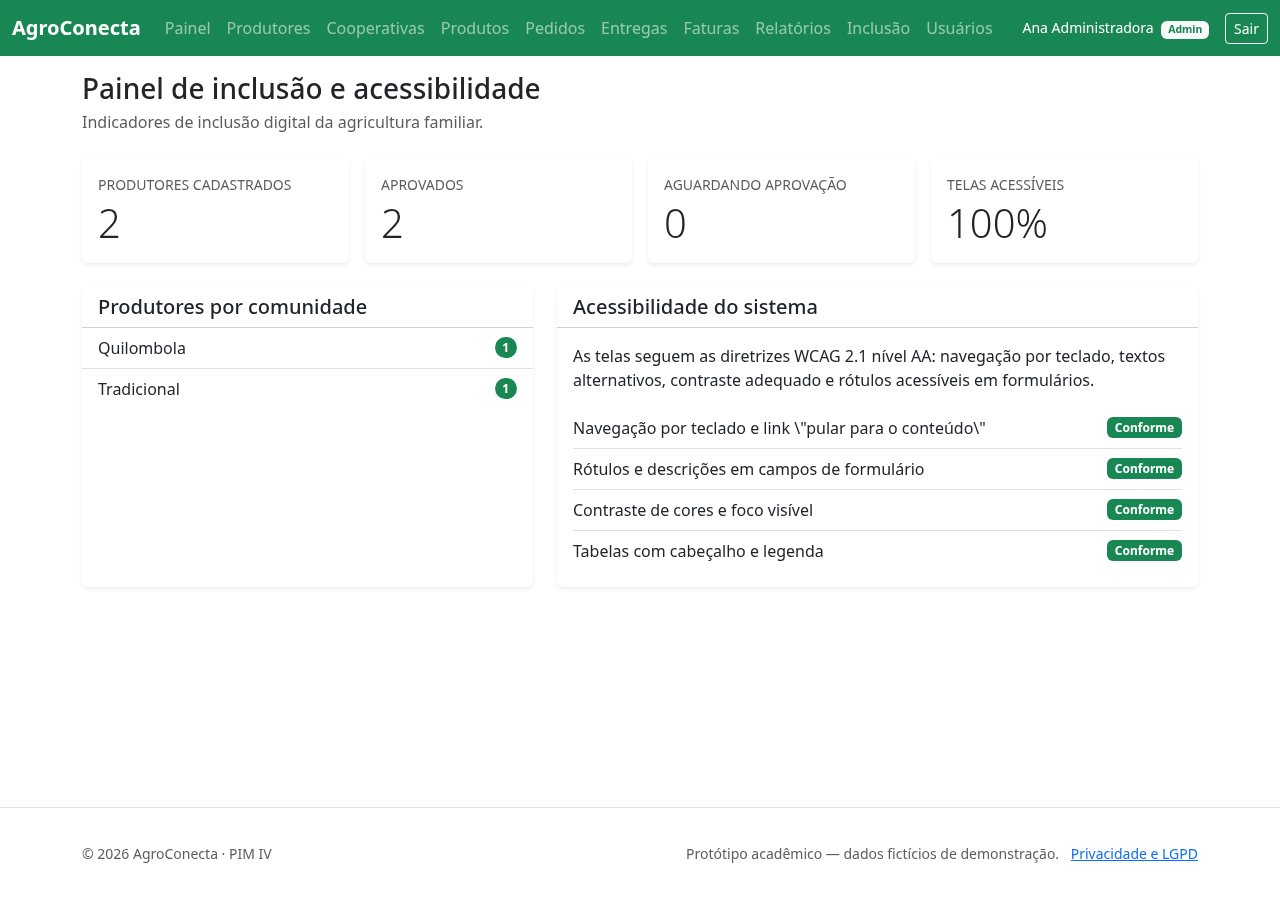
\includegraphics[width=0.92\textwidth]{figuras/inclusao.png}
  \fonte{elaborado pelo autor (2026)}
\end{figure}

\subsection{Combate à discriminação e valorização da diversidade}

O sistema adota o cadastro por comunidade -- tradicional, quilombola,
assentamento, indígena e outro -- não como mecanismo de segregação, mas de
reconhecimento e de formulação de políticas de fomento. A aprovação de cadastros
é realizada por um administrador, com registro em trilha de auditoria, o que
reduz a possibilidade de tratamento discriminatório e permite revisão das
decisões.

No plano operacional, a igualdade de acesso é garantida pelo uso em aparelhos
modestos e pela ausência de exigência de conexão permanente; no plano simbólico,
a nomenclatura e os exemplos reconhecem a contribuição das comunidades
tradicionais para a produção de alimentos.

\subsection{Acessibilidade}

As interfaces Web seguem as diretrizes WCAG 2.1 no nível AA (W3C, 2018). A
Tabela~\ref{tab:acessibilidade} relaciona os critérios aplicados e a forma de
implementação.

\begin{table}[H]
  \centering
  \caption{Critérios de acessibilidade aplicados}
  \label{tab:acessibilidade}
  \fontsize{10}{12}\selectfont
  \begin{tabular}{L{3.4cm}L{8.2cm}L{3.2cm}}
    \toprule
    \textbf{Critério} & \textbf{Implementação} & \textbf{Evidência} \\
    \midrule
    Idioma da página & Atributo \texttt{lang="pt-BR"} em todas as telas &
      Layout base \\
    Estrutura e relações & Tabelas com \texttt{caption}, \texttt{thead} e
      \texttt{scope}; formulários com rótulos associados & Telas de cadastro \\
    Contraste & Paleta com verde escuro sobre branco e foco visível &
      Folha de estilo \\
    Navegação por teclado & Ordem lógica de tabulação e link ``Pular para o
      conteúdo'' & Layout base \\
    Título da página & Título específico em cada tela & Controladores MVC \\
    Mensagens de erro & Texto descritivo junto ao campo, sem depender de cor &
      Validações \\
    Nome, função e valor & Controles nativos e \texttt{aria-label} quando
      necessário & Componentes \\
    \bottomrule
  \end{tabular}

  \vspace{2pt}
  {\fontsize{10}{12}\selectfont\itshape Fonte: elaborado pelo autor (2026), com
  base em W3C (2018)}
\end{table}

No aplicativo mobile, foram aplicados rótulos acessíveis nos botões, suporte a
escala de fonte do sistema, contraste adequado, alvos de toque com pelo menos
44 pontos e títulos semânticos de tela. A matriz de testes registra a verificação
manual com leitor de tela e as limitações encontradas, discutidas na seção 5.6.

\subsection{Proteção de dados e cidadania digital}

A plataforma trata dados pessoais de produtores, compradores e motoristas, ainda
que em contexto acadêmico e com dados fictícios. Por isso, foram adotadas medidas
alinhadas à Lei Geral de Proteção de Dados (BRASIL, 2018): finalidade e
minimização (apenas dados necessários à operação), segurança (senhas com PBKDF2,
HTTPS, autorização por papel), transparência (página pública de privacidade,
Figura~\ref{fig:privacidade}), direitos do titular (canal de contato e
possibilidade de correção) e prestação de contas (trilha de auditoria).

\begin{figure}[H]
  \centering
  \caption{Página pública de política de privacidade}
  \label{fig:privacidade}
  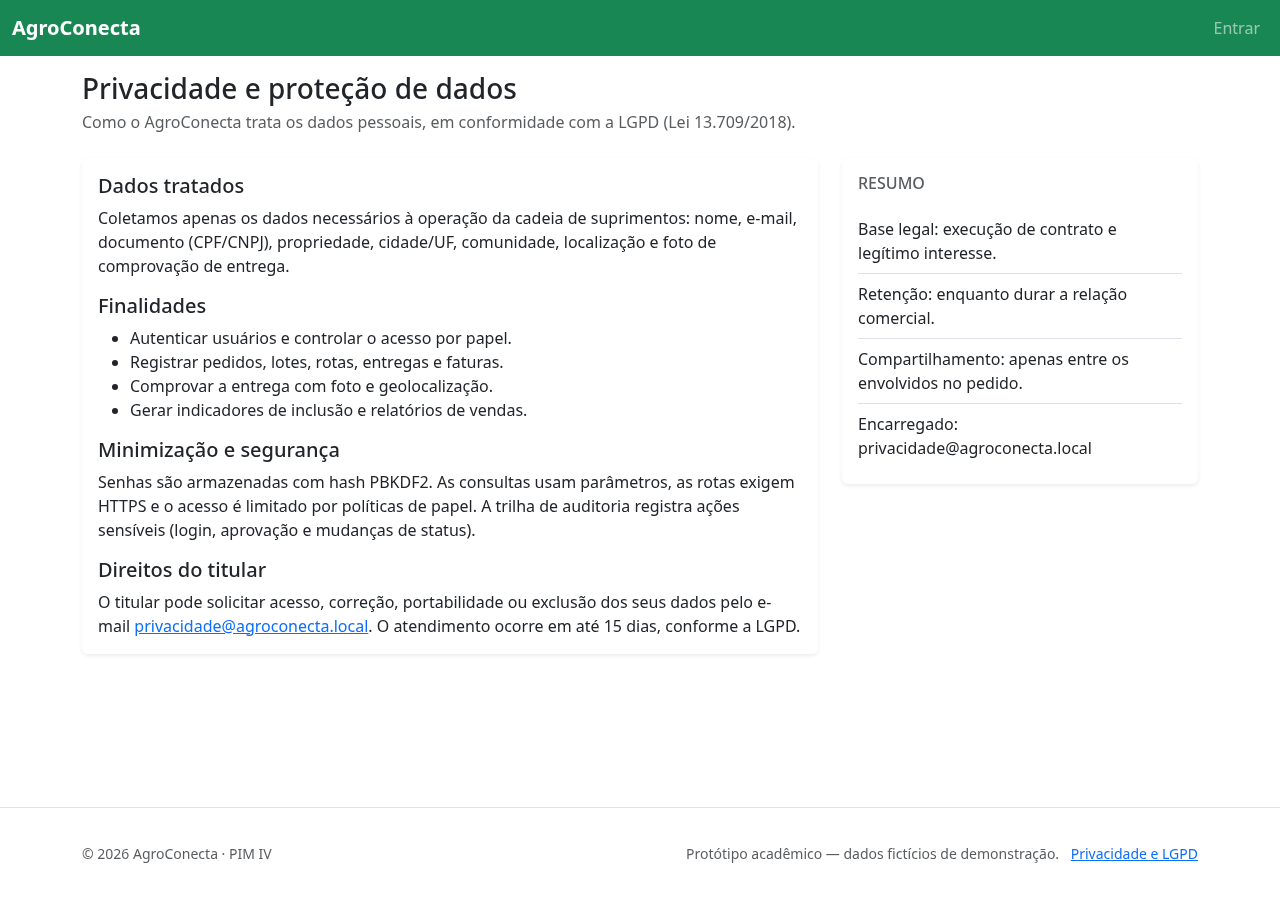
\includegraphics[width=0.92\textwidth]{figuras/privacidade.png}
  \fonte{elaborado pelo autor (2026)}
\end{figure}

\subsection{Contribuição para os Objetivos de Desenvolvimento Sustentável}

A solução dialoga com a Agenda 2030 (ONU, 2015) em três objetivos. O ODS 2
(fome zero) é apoiado pela redução de perdas e pela melhoria do escoamento da
produção. O ODS 8 (trabalho decente e crescimento econômico) é atendido pela
ampliação do acesso a mercados institucionais e pela formalização das
transações. O ODS 10 (redução das desigualdades) é endereçado pela inclusão
digital de comunidades tradicionais e pela transparência na distribuição dos
repiques financeiros entre os associados.

% ============================================================================
% Capítulo 4 — Desenvolvimento da solução Web
% ============================================================================
\section{DESENVOLVIMENTO DA SOLUÇÃO WEB}

\subsection{Visão geral}

A aplicação Web foi construída em ASP.NET Core 10, com o padrão
Model-View-Controller (MVC) para as telas administrativas e uma camada de API
REST versionada para o consumo pelo aplicativo mobile e por integrações futuras.
A mesma solução hospeda as duas superfícies: o navegador recebe páginas
renderizadas no servidor, enquanto o aplicativo consome JSON sob o prefixo
\texttt{/api/v1}. Essa decisão reduz o custo operacional de manter dois
artefatos e garante que regras de negócio sejam aplicadas uma única vez.

A interface utiliza Bootstrap 5 com identidade visual própria, baseada em tons de
verde, tipografia legível e formulários com validação no cliente e no servidor.
Todas as páginas compartilham um layout com menu lateral, área de conteúdo
principal, mensagens de retorno e link de acessibilidade para saltar diretamente
ao conteúdo.

\subsection{Arquitetura e organização}

O projeto Web é dividido em controladores MVC, controladores de API, view models,
visões Razor e serviços de apresentação. A Tabela~\ref{tab:telas} relaciona as
telas implementadas, a rota de acesso e o público autorizado.

\begin{table}[H]
  \centering
  \caption{Telas da aplicação Web}
  \label{tab:telas}
  \fontsize{9}{11}\selectfont
  \begin{tabular}{L{3.4cm}L{3.6cm}L{5.4cm}L{2.2cm}}
    \toprule
    \textbf{Tela} & \textbf{Rota} & \textbf{Função} & \textbf{Perfil} \\
    \midrule
    Login & \texttt{/Account/Login} & Autenticação por cookie & Público \\
    Painel & \texttt{/} & Indicadores e atalhos & Todos \\
    Produtores & \texttt{/Produtores} & Cadastro e aprovação & Admin \\
    Cooperativas & \texttt{/Cooperativas} & Cadastro de cooperativas & Admin \\
    Produtos & \texttt{/ProdutosWeb} & Catálogo e preços & Admin \\
    Pedidos & \texttt{/PedidosWeb} & Lista, detalhe e status & Admin, Comprador \\
    Entregas e rotas & \texttt{/EntregasWeb} & Rotas, entregas e nova rota & Admin, Motorista \\
    Faturas & \texttt{/Faturas} & Emissão e consulta & Admin \\
    Relatórios & \texttt{/Relatorios/}\allowbreak\texttt{VendasPorProdutor} & Vendas por produtor & Admin \\
    Inclusão & \texttt{/Inclusao} & Produtores por comunidade & Admin \\
    Usuários & \texttt{/Usuarios} & Contas e papéis & Admin \\
    Auditoria & \texttt{/Usuarios/Auditoria} & Trilha de ações & Admin \\
    Privacidade & \texttt{/Home/Privacidade} & Política de dados & Público \\
    \bottomrule
  \end{tabular}

  \vspace{2pt}
  {\fontsize{10}{12}\selectfont\itshape Fonte: elaborado pelo autor (2026)}
\end{table}

A Figura~\ref{fig:painel} apresenta o painel principal, que reúne indicadores de
produtores ativos, pedidos em aberto, entregas pendentes e faturamento do
período, além de atalhos para as operações mais frequentes.

\begin{figure}[H]
  \centering
  \caption{Painel principal da aplicação Web}
  \label{fig:painel}
  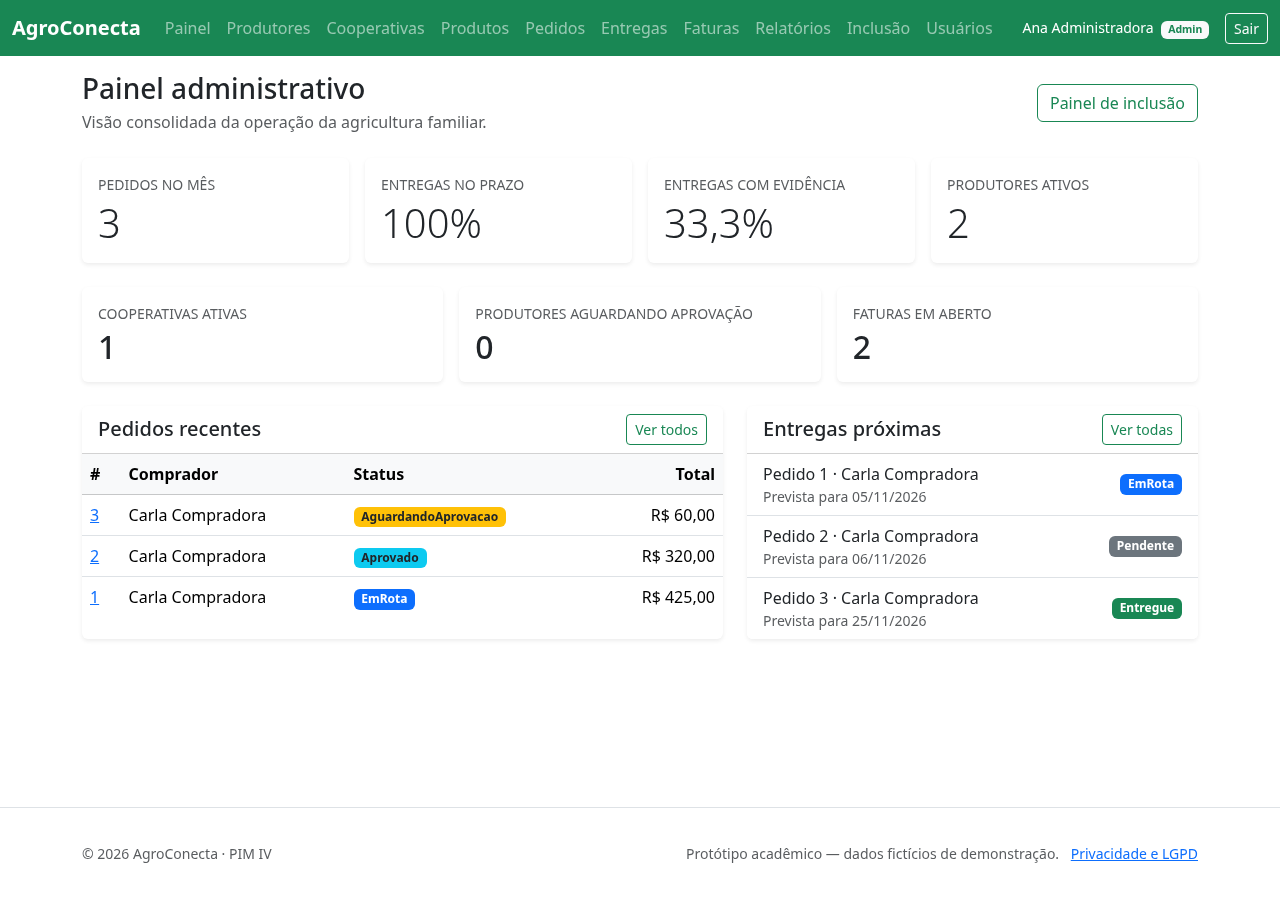
\includegraphics[width=0.80\textwidth]{figuras/painel.png}
  \fonte{elaborado pelo autor (2026)}
\end{figure}

\subsection{Autenticação e controle de acesso}

A autenticação Web utiliza cookie seguro emitido pelo ASP.NET Core Identity,
com proteção antiforgery em todos os formulários POST. As políticas de
autorização são declaradas por papel: \texttt{SomenteAdmin},
\texttt{GerenciarCatalogo}, \texttt{Comprar}, \texttt{OperarPedidos} e
\texttt{Entregar}. O escopo dos dados também é verificado: um comprador só
acessa seus próprios pedidos e recebe resposta 404 -- e não 403 -- ao tentar
consultar recurso de terceiros, evitando a exposição da existência do registro.

\subsection{Cadastros e operação}

Os cadastros de produtores, cooperativas e produtos utilizam formulários com
validação declarativa e mensagens em português, com listagens que exibem a
situação do cadastro e a comunidade de origem.

A operação de pedidos concentra o fluxo comercial. A Figura~\ref{fig:pedidos}
apresenta a listagem com filtros por status e o detalhe do pedido, que exibe
itens, lote de origem, endereço de entrega e histórico de status.

\begin{figure}[H]
  \centering
  \caption{Gestão de pedidos}
  \label{fig:pedidos}
  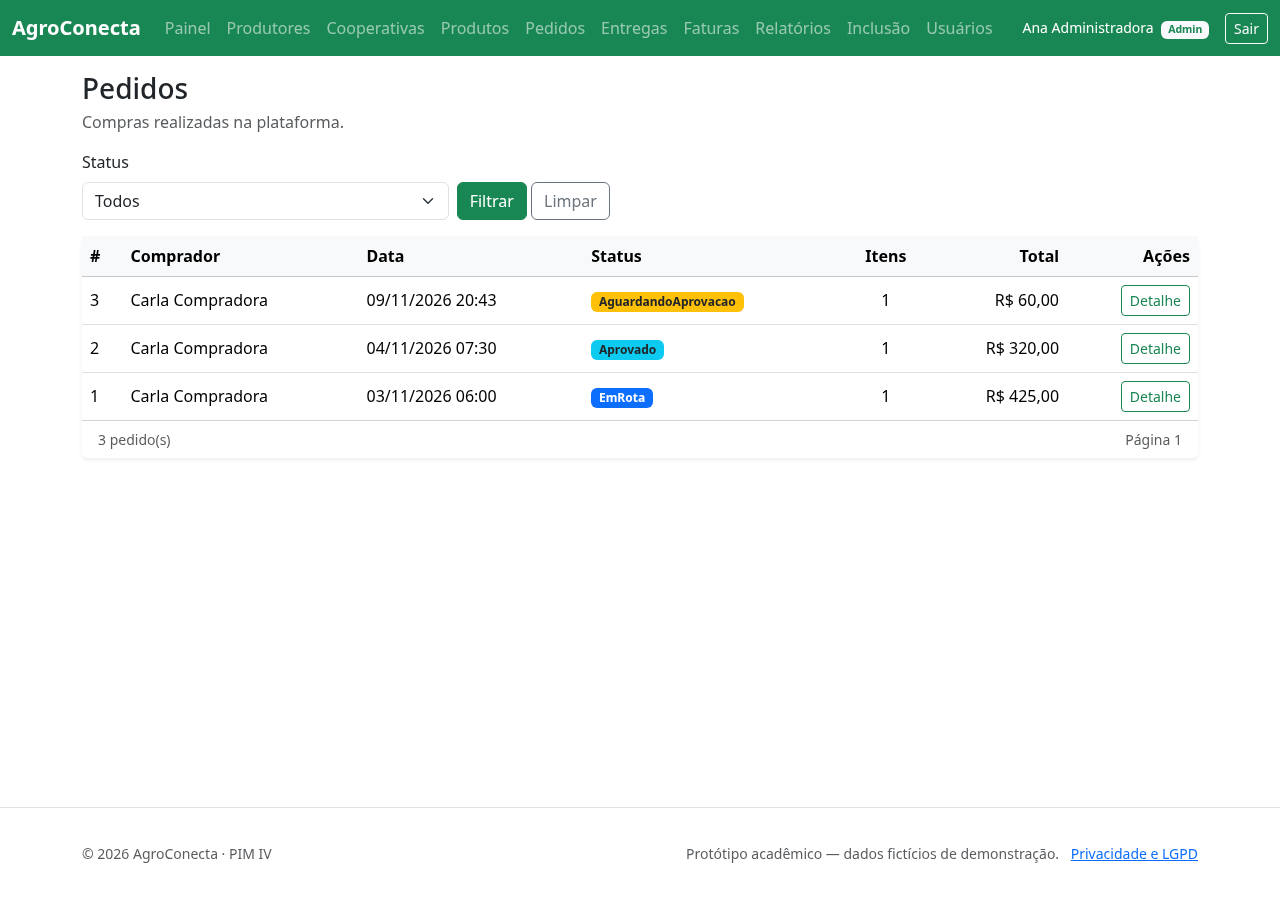
\includegraphics[width=0.80\textwidth]{figuras/pedidos.png}
  \fonte{elaborado pelo autor (2026)}
\end{figure}

As entregas são agrupadas em rotas. Cada rota possui data, motorista, veículo e
um conjunto de pedidos; ao ser criada, gera automaticamente uma entrega por
pedido, conforme a Figura~\ref{fig:entregas}.

\begin{figure}[H]
  \centering
  \caption{Entregas e rotas programadas}
  \label{fig:entregas}
  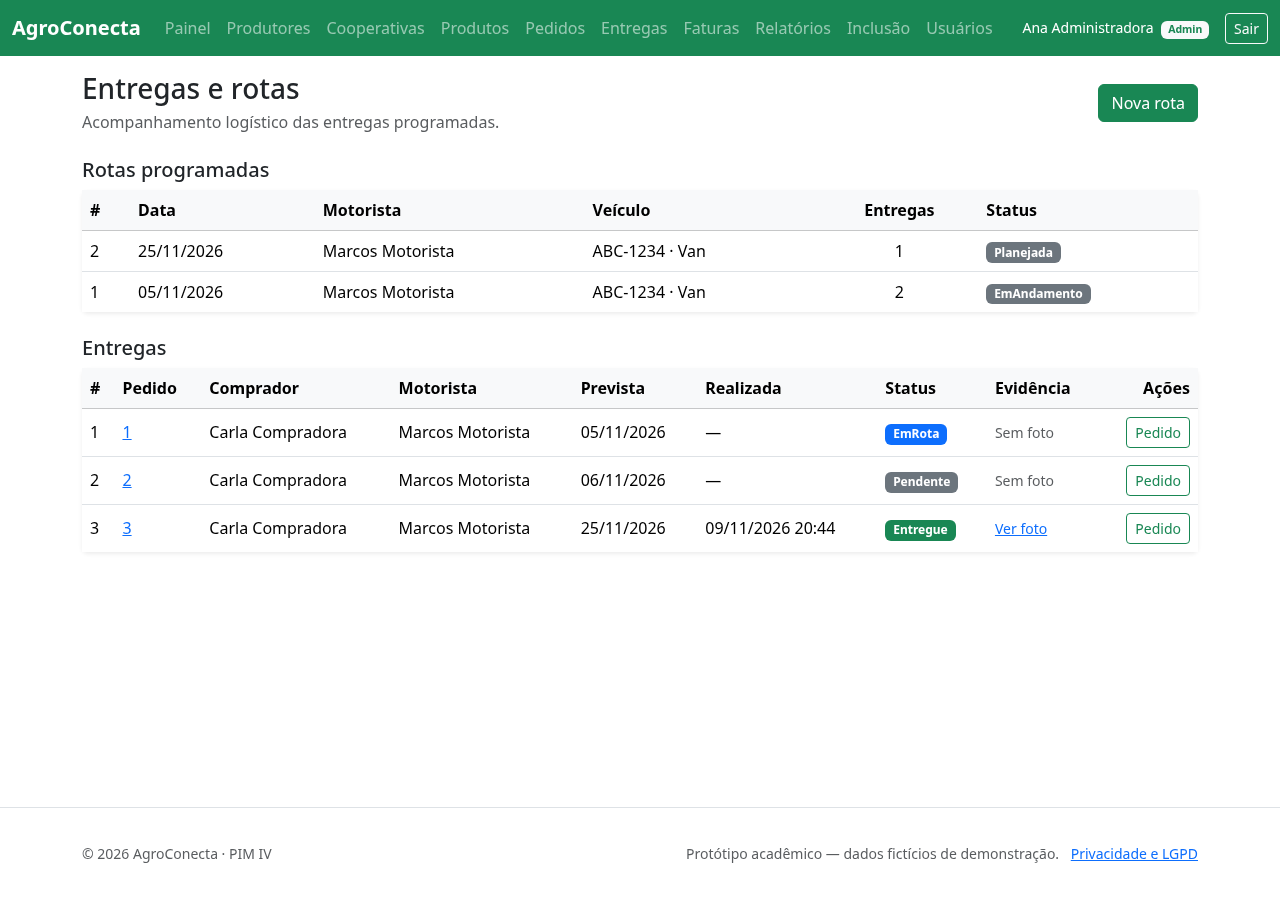
\includegraphics[width=0.80\textwidth]{figuras/entregas.png}
  \fonte{elaborado pelo autor (2026)}
\end{figure}

O faturamento é realizado a partir do pedido, com geração idempotente: se a
fatura já existir, a operação retorna o registro existente em vez de duplicá-lo.
A numeração segue o padrão \texttt{FAT-ANO-SEQUENCIAL}, como ilustrado na
Figura~\ref{fig:faturas}.

\begin{figure}[H]
  \centering
  \caption{Consulta e emissão de faturas}
  \label{fig:faturas}
  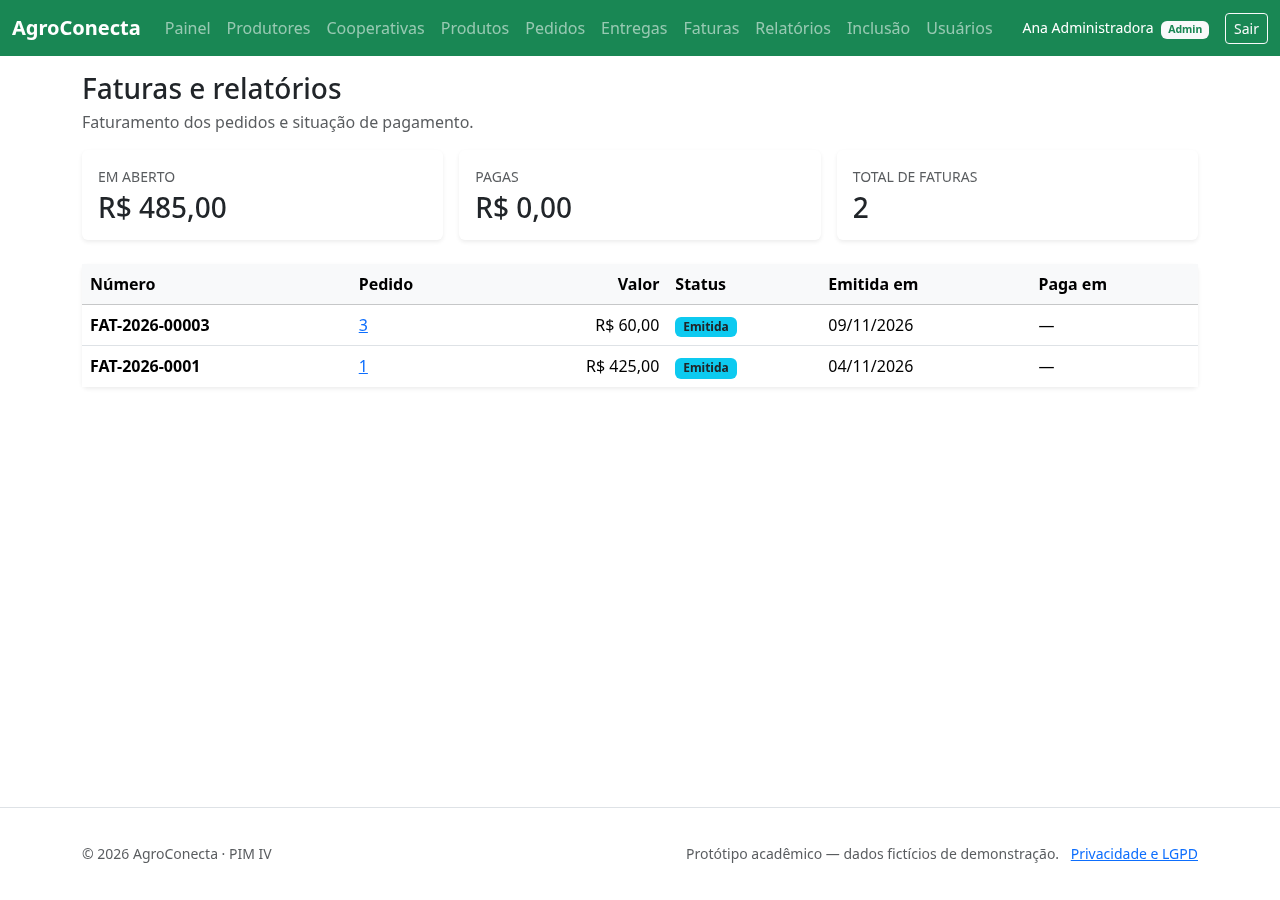
\includegraphics[width=0.80\textwidth]{figuras/faturas.png}
  \fonte{elaborado pelo autor (2026)}
\end{figure}

\subsection{Relatórios e indicadores}

O relatório de vendas por produtor consolida, por período, a quantidade
comercializada e o valor total de cada associado, permitindo comparar
comunidades e orientar políticas de crédito e fomento. A consulta é executada
por procedimento armazenado no banco, o que reduz o tráfego de dados e aproveita
a capacidade de agregação do SGBD. A Figura~\ref{fig:relatorios} apresenta o
resultado com dados de demonstração.

\begin{figure}[H]
  \centering
  \caption{Relatório de vendas por produtor}
  \label{fig:relatorios}
  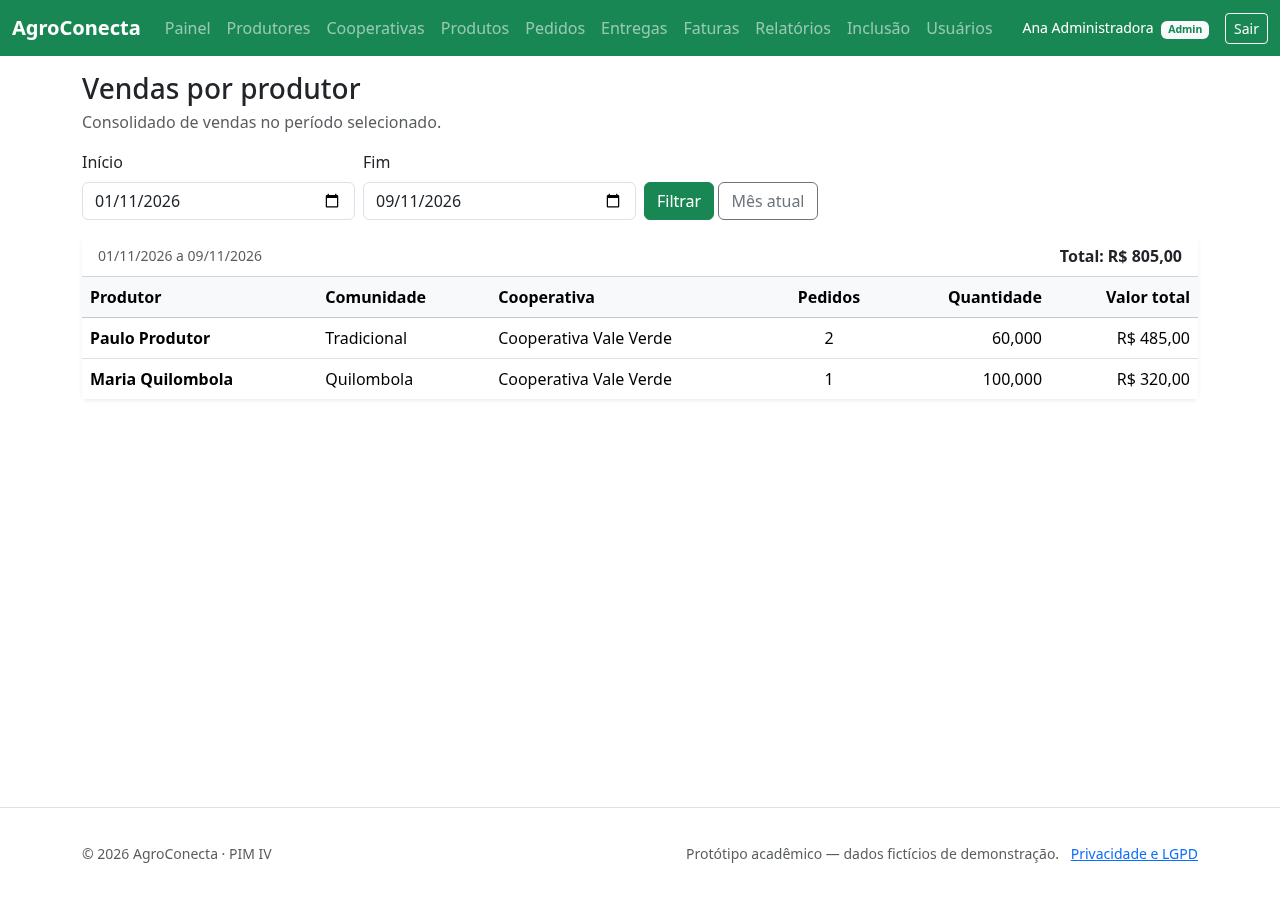
\includegraphics[width=0.80\textwidth]{figuras/relatorios.png}
  \fonte{elaborado pelo autor (2026)}
\end{figure}

Além do relatório, a API expõe um endpoint de indicadores que alimenta o painel
e o aplicativo: número de produtores ativos, pedidos no período, entregas
pendentes, faturamento e percentual de telas acessíveis. Os valores são
calculados no servidor, garantindo consistência entre Web e mobile.

\subsection{API REST e contrato}

A API é versionada em \texttt{/api/v1}, documentada com OpenAPI 3.0 e protegida
por JWT com token de acesso de curta duração e refresh token separado. Os erros
seguem o padrão RFC 7807 (\emph{Problem Details}), com identificador de
correlação para rastreamento. A Tabela~\ref{tab:endpoints} lista os caminhos
publicados.

\begin{table}[H]
  \centering
  \caption{Endpoints da API}
  \label{tab:endpoints}
  \fontsize{9}{11}\selectfont
  \begin{tabular}{L{6.8cm}L{2.2cm}L{6.0cm}}
    \toprule
    \textbf{Caminho} & \textbf{Métodos} & \textbf{Finalidade} \\
    \midrule
    \texttt{/health} & GET & Estado da aplicação \\
    \texttt{/api/v1/auth/login} & POST & Autenticação e emissão de tokens \\
    \texttt{/api/v1/auth/refresh} & POST & Renovação do token de acesso \\
    \texttt{/api/v1/auth/logout} & POST & Encerramento da sessão \\
    \texttt{/api/v1/me} & GET & Perfil do usuário autenticado \\
    \texttt{/api/v1/produtos} & GET, POST & Catálogo \\
    \texttt{/api/v1/produtos/\{id\}} & GET, PUT, DELETE & Manutenção de produto \\
    \texttt{/api/v1/lotes} & GET, POST & Lotes de colheita \\
    \texttt{/api/v1/lotes/meus} & GET & Lotes do produtor autenticado \\
    \texttt{/api/v1/lotes/\{id\}} & GET & Detalhe do lote \\
    \texttt{/api/v1/pedidos} & GET, POST & Pedidos \\
    \texttt{/api/v1/pedidos/\{id\}} & GET & Detalhe do pedido \\
    \texttt{/api/v1/pedidos/\{id\}/status} & PATCH & Transição de status \\
    \texttt{/api/v1/entregas/minhas} & GET & Entregas do motorista \\
    \texttt{/api/v1/entregas/\{id\}/status} & PATCH & Atualização de entrega \\
    \texttt{/api/v1/entregas/\{id\}/evidencia} & PUT & Evidência multipart \\
    \texttt{/api/v1/rotas} & GET, POST & Rotas e geração de entregas \\
    \texttt{/api/v1/faturas} & GET & Consulta de faturas \\
    \texttt{/api/v1/faturas/pedido/\{pedidoId\}} & POST & Emissão idempotente \\
    \texttt{/api/v1/indicadores} & GET & Indicadores do painel \\
    \texttt{/api/v1/relatorios/vendas-produtor} & GET & Relatório por período \\
    \texttt{/api/v1/auditoria} & GET & Trilha de auditoria \\
    \bottomrule
  \end{tabular}

  \vspace{2pt}
  {\fontsize{9}{11}\selectfont\itshape Fonte: elaborado pelo autor (2026)}
\end{table}

O contrato OpenAPI é mantido em \texttt{contracts/} e tratado como fonte de
verdade: alterações são feitas primeiro nele, depois na implementação e, por fim,
na geração dos tipos TypeScript do aplicativo, disciplina que evitou divergências
entre as duas superfícies.

% ============================================================================
% Capítulo 5 — Desenvolvimento da solução Mobile
% ============================================================================
\section{DESENVOLVIMENTO DA SOLUÇÃO MOBILE}

\subsection{Objetivo e tecnologias}

O aplicativo AgroConecta Mobile foi desenvolvido para dois perfis que atuam
diretamente no campo: o produtor, que registra a colheita, e o motorista, que
atualiza as entregas e comprova a entrega. A base tecnológica é React Native
0.88 com Expo SDK 58 (EXPO, 2026; REACT NATIVE, 2026) e TypeScript, o que permite um único código para Android e
iOS, acesso simplificado a recursos nativos (câmera, localização, armazenamento)
e distribuição por APK ou pelas lojas oficiais.

A escolha do TypeScript não é apenas estilística: os tipos das respostas da API
são gerados a partir do contrato OpenAPI, de modo que qualquer alteração no
contrato produz erro de compilação no aplicativo antes de chegar ao aparelho.
Esse mecanismo foi decisivo para manter as duas frentes de desenvolvimento
alinhadas.

\subsection{Telas e fluxo de navegação}

O aplicativo organiza-se em uma pilha de autenticação e duas abas principais,
uma para cada perfil. A Tabela~\ref{tab:telasmobile} descreve as telas
implementadas.

\begin{table}[H]
  \centering
  \caption{Telas do aplicativo mobile}
  \label{tab:telasmobile}
  \fontsize{9.5}{11.5}\selectfont
  \begin{tabular}{L{3.4cm}L{3.0cm}L{8.6cm}}
    \toprule
    \textbf{Tela} & \textbf{Perfil} & \textbf{Função} \\
    \midrule
    Login & Ambos & Autenticação e armazenamento seguro da sessão \\
    Início & Ambos & Resumo de lotes ou entregas do usuário \\
    Meus lotes & Produtor & Lista com situação de sincronização \\
    Novo lote & Produtor & Registro de produto, quantidade e data de colheita \\
    Detalhe do lote & Produtor & Dados do lote e código de rastreio \\
    Minhas entregas & Motorista & Lista de entregas por status \\
    Detalhe da entrega & Motorista & Pedido, comprador, endereço e itens \\
    Status da entrega & Motorista & Transições permitidas, com data e hora \\
    Evidência & Motorista & Câmera ou galeria, GPS e observação \\
    Perfil & Ambos & Dados do usuário, sincronização e logout \\
    \bottomrule
  \end{tabular}

  \vspace{2pt}
  {\fontsize{10}{12}\selectfont\itshape Fonte: elaborado pelo autor (2026)}
\end{table}

O fluxo de navegação é apresentado na Figura~\ref{fig:navmobile}. A aba exibida
depende do papel do usuário autenticado, evitando que o produtor visualize
funções de entrega e vice-versa.

\begin{figure}[H]
  \centering
  \caption{Fluxo de navegação do aplicativo}
  \label{fig:navmobile}
  \begin{tikzpicture}[
    tela/.style={draw, rounded corners=3pt, align=center, font=\fontsize{8.5}{10}\selectfont,
      minimum height=8mm, text width=26mm, inner sep=2.5pt},
    seta/.style={-latex, thin}
  ]
    \node[tela] (login) at (0,0) {Login};
    \node[tela] (inicio) at (0,-1.5) {Início (por papel)};
    \node[tela] (lotes) at (-5.0,-3.2) {Meus lotes};
    \node[tela] (novo) at (-5.9,-4.9) {Novo lote};
    \node[tela] (dlote) at (-2.3,-4.9) {Detalhe do lote};
    \node[tela] (entregas) at (1.2,-3.2) {Minhas entregas};
    \node[tela] (dent) at (1.2,-4.9) {Detalhe da entrega};
    \node[tela] (status) at (-1.0,-6.6) {Status};
    \node[tela] (evid) at (2.2,-6.6) {Evidência};
    \node[tela] (perfil) at (5.4,-1.5) {Perfil e\\ sincronização};

    \draw[seta] (login) -- (inicio);
    \draw[seta] (inicio) -- (lotes);
    \draw[seta] (lotes) -- (novo);
    \draw[seta] (lotes) -- (dlote);
    \draw[seta] (inicio) -- (entregas);
    \draw[seta] (entregas) -- (dent);
    \draw[seta] (dent) -- (status);
    \draw[seta] (dent) -- (evid);
    \draw[seta] (inicio) -- (perfil);
  \end{tikzpicture}
  \fonte{elaborado pelo autor (2026)}
\end{figure}

\subsection{Autenticação e sessão}

O login consome o mesmo endpoint da API utilizada pela Web. Os tokens são
armazenados no \texttt{expo-secure-store}, que utiliza o armazenamento
criptográfico do sistema operacional, e não em armazenamento comum. Um
interceptador renova o token de acesso de forma transparente quando recebe 401 e
redireciona ao login apenas quando a renovação falha. No logout, os tokens e os
dados sensíveis da sessão são removidos.

\subsection{Operação offline e sincronização}

O requisito mais desafiador do aplicativo é operar sem conexão. A estratégia
combina três componentes: banco local em SQLite, fila de operações pendentes e
serviço de sincronização acionado pela mudança de conectividade.

Quando o produtor registra um lote sem sinal, o aplicativo grava o registro
localmente com estado \emph{pendente} e enfileira a operação. Quando o motorista
atualiza o status ou anexa uma evidência, o mesmo mecanismo é acionado. Ao
detectar reconexão, o serviço processa a fila em ordem, com recuo exponencial em
caso de falha temporária e limite de tentativas. A Figura~\ref{fig:sync} ilustra
o ciclo.

\begin{figure}[H]
  \centering
  \caption{Ciclo de sincronização offline}
  \label{fig:sync}
  \begin{tikzpicture}[
    nodo/.style={draw, rounded corners=3pt, align=center, font=\fontsize{8}{9}\selectfont,
      minimum height=9mm, text width=24mm, inner sep=2pt},
    seta/.style={-latex, thin},
    rotulo/.style={font=\fontsize{8}{9}\selectfont, fill=white, inner sep=1pt}
  ]
    \node[nodo] (local) at (1.5,0) {Operação local\\(SQLite)};
    \node[nodo] (fila)  at (5.9,0) {Fila de\\ pendências};
    \node[nodo] (envio) at (10.3,0) {Envio à API};
    \node[nodo] (ok)    at (14.4,0) {Sincronizado};

    \node[nodo] (erro)     at (5.9,-3.1) {Falha temporária\\(recuo exponencial)};
    \node[nodo] (conflito) at (10.3,-3.1) {Conflito 409\\(visível ao usuário)};

    \draw[seta] (local) -- node[rotulo, above] {enfileira} (fila);
    \draw[seta] (fila) -- node[rotulo, above] {reconexão} (envio);
    \draw[seta] (envio) -- node[rotulo, above] {2xx} (ok);
    \draw[seta] (envio) -- node[rotulo, right] {409} (conflito);
    \draw[seta] (envio.south west) -- node[rotulo, above left] {5xx} (erro.east);
    \draw[seta] (erro) -- node[rotulo, left] {retenta} (fila);
  \end{tikzpicture}
  \fonte{elaborado pelo autor (2026)}
\end{figure}

O conflito é tratado como evento de negócio, não como erro genérico: quando o
servidor responde 409 porque o lote já foi sincronizado ou porque o status da
entrega mudou, o aplicativo marca o item como conflitante, interrompe as
tentativas automáticas e exibe a situação ao usuário. Essa decisão evita o
fenômeno de ``fila infinita'' e preserva a confiança nos dados.

\subsection{Evidência de entrega}

A evidência é composta por três elementos: fotografia, coordenadas geográficas e
observação textual. A foto pode ser capturada pela câmera ou escolhida na
galeria; antes do envio, é redimensionada e comprimida para reduzir o consumo de
dados. A localização é obtida com permissão explícita do usuário e validada
quanto à faixa de latitude e longitude.

O envio utiliza requisição multipart nativa do sistema, por meio de
\texttt{FileSystem.}\allowbreak\texttt{uploadAsync}, solução adotada após identificar que o envio
via \texttt{fetch} falhava em determinados aparelhos Android antes de atingir o
servidor. O contrato permaneceu o mesmo (\texttt{PUT
/api/v1/entregas/\{id\}/evidencia}), alterando apenas o mecanismo de transporte.
O arquivo é armazenado no servidor com nome gerado, sem confiar no nome enviado
pelo cliente.

\subsection{Testes, integração e limitações}

O aplicativo conta com 17 suítes e 79 testes automatizados, cobrindo componentes
de interface, validações, armazenamento local, fila de sincronização, conflitos e
chamadas de API. A verificação de qualidade é executada por um único comando, que
reúne análise estática, verificação de tipos e testes.

A integração real foi validada em aparelho Android 13, com a API executando
contra SQL Server e redirecionamento de porta por USB. O fluxo completo --
login do produtor, criação de lote, login do motorista, atualização de entrega e
envio de evidência com foto e GPS -- foi executado com persistência confirmada no
banco. O APK de release foi gerado com o pacote JavaScript embutido e instalado
no aparelho, funcionando sem o servidor de desenvolvimento.

Como limitações, o APK validado contempla apenas a arquitetura
\texttt{arm64-v8a}, a validação com leitor de tela TalkBack foi parcial e a
distribuição pelo EAS não foi executada por ausência de credenciais. Nenhuma
delas afeta o fluxo funcional, mas todas devem ser tratadas antes de uma
publicação em produção.

% ============================================================================
% Capítulo 6 — Arquitetura de software
% ============================================================================
\section{ARQUITETURA DE SOFTWARE}

\subsection{Estilo arquitetural}

A solução adota o estilo de \textbf{monólito modular em camadas}, com separação
rígida de dependências: o domínio não conhece infraestrutura, a aplicação
depende apenas do domínio e a infraestrutura implementa as abstrações definidas
nas camadas internas. Essa organização segue os princípios de inversão de
dependência e permite substituir detalhes tecnológicos -- banco, armazenamento de
arquivos, provedor de tokens -- sem alterar as regras de negócio (MARTIN, 2017;
EVANS, 2003).

A escolha por um monólito modular, em vez de microsserviços, é deliberada. O
volume de operações da cooperativa não justifica a complexidade operacional de
serviços distribuídos, e a equipe reduzida teria dificuldade de sustentar
múltiplas implantações. O monólito modular preserva a possibilidade de extração
futura de módulos, caso o crescimento o exija, sem pagar antecipadamente o custo
de coordenação distribuída.

\begin{figure}[H]
  \centering
  \caption{Arquitetura em camadas da solução (a seta à direita representa a inversão de dependência)}
  \label{fig:camadas}
  \begin{tikzpicture}[
    camada/.style={draw, rounded corners=3pt, minimum width=130mm, minimum height=13mm,
      align=center, font=\fontsize{9.5}{11}\selectfont},
    seta/.style={-latex, thick, gray!70}
  ]
    \node[camada, fill=blue!8] (apres) {\textbf{Apresentação} --- MVC, Web API, Swagger, views Razor};
    \node[camada, fill=green!8, below=3mm of apres] (aplic) {\textbf{Aplicação} --- casos de uso, validações, DTOs, autorização};
    \node[camada, fill=orange!10, below=3mm of aplic] (dom) {\textbf{Domínio} --- entidades, enums, invariantes, contratos de repositório};
    \node[camada, fill=gray!10, below=3mm of dom] (infra) {\textbf{Infraestrutura} --- EF Core, SQL Server, JWT, arquivos, seed};
    \draw[seta] (apres) -- (aplic);
    \draw[seta] (aplic) -- (dom);
    \draw[seta] (infra.east) -- ++(1.4,0) |- (dom.east);
  \end{tikzpicture}
  \fonte{elaborado pelo autor (2026)}
\end{figure}

\subsection{Camadas e responsabilidades}

A Tabela~\ref{tab:camadas} detalha o papel de cada projeto da solução e os
artefatos que concentra.

\begin{table}[H]
  \centering
  \caption{Camadas, projetos e responsabilidades}
  \label{tab:camadas}
  \fontsize{9.5}{11.5}\selectfont
  \begin{tabular}{L{2.4cm}L{4.5cm}L{7.9cm}}
    \toprule
    \textbf{Camada} & \textbf{Projeto} & \textbf{Responsabilidade} \\
    \midrule
    Domínio & \texttt{AgroConecta.Domain} & Entidades, enums, invariantes,
      contratos de repositório e unidade de trabalho \\
    Aplicação & \texttt{AgroConecta.Application} & Casos de uso, comandos,
      consultas, validações e regras de orquestração \\
    Infraestrutura & \texttt{AgroConecta.Infrastructure} & Contexto EF Core,
      mapeamentos, repositórios, migrations, seed e serviços técnicos \\
    Apresentação & \texttt{AgroConecta.Web} & Controladores MVC, API REST,
      views, filtros, middlewares e configuração \\
    Testes & \texttt{AgroConecta.Tests} & Testes unitários, de integração e de
      API \\
    \bottomrule
  \end{tabular}

  \vspace{2pt}
  {\fontsize{10}{12}\selectfont\itshape Fonte: elaborado pelo autor (2026)}
\end{table}

\subsection{Orientação a objetos e princípios SOLID}

O modelo de domínio utiliza classes com estado protegido e comportamento
explícito. Todas as entidades herdam de \texttt{EntidadeBase}, que concentra
identificador, datas de criação e atualização e a comparação por identidade --
evitando duplicação e garantindo consistência transversal. As transições de
estado são implementadas como métodos, e não como atribuições diretas: uma
entrega só pode ser marcada como concluída se estiver em rota, e um pedido só
pode ser cancelado enquanto não houver fatura emitida. Essa abordagem mantém as
invariantes próximas dos dados que protegem.

Os princípios SOLID estão presentes de forma concreta: a
\textbf{responsabilidade única} separa entidade, caso de uso e repositório; o
\textbf{aberto/fechado} permitiu incluir rotas e faturamento sem alterar
entidades existentes; a \textbf{segregação de interfaces} mantém um contrato por
agregado; e a \textbf{inversão de dependência} sustenta a arquitetura, com a
aplicação declarando o que precisa e a infraestrutura fornecendo a
implementação.

\subsection{Padrões aplicados}

A Tabela~\ref{tab:padroes} resume os padrões utilizados e sua justificativa no
contexto do projeto.

\begin{table}[H]
  \centering
  \caption{Padrões de projeto aplicados}
  \label{tab:padroes}
  \fontsize{9.5}{11.5}\selectfont
  \begin{tabular}{L{3.4cm}L{5.8cm}L{5.8cm}}
    \toprule
    \textbf{Padrão} & \textbf{Aplicação} & \textbf{Benefício} \\
    \midrule
    Repository & Interfaces no domínio, implementação com EF Core &
      Isola a persistência e facilita testes com dublês \\
    Unit of Work & \texttt{IUnidadeDeTrabalho} com transação única por caso de
      uso & Consistência entre agregados \\
    Caso de uso & Uma classe por operação (\texttt{CriarPedido},
      \texttt{GerarFatura}) & Regras explícitas e testáveis \\
    DTO & Contratos de entrada e saída separados das entidades & Evita
      exposição do modelo interno \\
    Result & Retorno explícito de sucesso ou falha de negócio & Erros
      previsíveis sem exceções de controle de fluxo \\
    Problem Details & Respostas de erro padronizadas (RFC 7807) & Integração
      simples para o cliente mobile \\
    \bottomrule
  \end{tabular}

  \vspace{2pt}
  {\fontsize{10}{12}\selectfont\itshape Fonte: elaborado pelo autor (2026)}
\end{table}

\subsection{Modularização e dependências}

A solução é organizada em uma solução única com seis projetos, cujas referências
apontam sempre para dentro: \texttt{Web} depende de \texttt{Application} e
\texttt{Infrastructure}; \texttt{Infrastructure} depende de
\texttt{Application} e \texttt{Domain}; \texttt{Application} depende apenas de
\texttt{Domain}; e \texttt{Domain} não depende de nenhum outro projeto. Os
testes referenciam todas as camadas, mas não são referenciados por nenhuma.

Essa disciplina produz dois efeitos práticos. Primeiro, impede que detalhes de
banco contaminem as regras de negócio. Segundo, torna o domínio e a aplicação
plenamente testáveis sem servidor ou banco, o que explica a cobertura de 92,5\%
e 93,8\% nessas camadas, respectivamente, com 159 testes automatizados. A
verificação de arquitetura é feita pelo compilador: qualquer referência
indevida quebra o build, e não apenas uma convenção de equipe.

% ============================================================================
% Capítulo 7 — Projeto do banco de dados
% ============================================================================
\section{PROJETO DO BANCO DE DADOS}

\subsection{Modelo de dados}

O banco de dados foi modelado em SQL Server 2022 e é composto por quatorze
tabelas de negócio, além da tabela de controle de migrations. O modelo segue a
terceira forma normal: cada fato é armazenado uma única vez, e as relações são
expressas por chaves estrangeiras com integridade referencial explícita. A
Tabela~\ref{tab:entidades} descreve as entidades e seu papel no domínio.

\begin{table}[H]
  \centering
  \caption{Entidades do modelo de dados}
  \label{tab:entidades}
  \fontsize{9.5}{11.5}\selectfont
  \begin{tabular}{L{3.4cm}L{11.6cm}}
    \toprule
    \textbf{Entidade} & \textbf{Descrição} \\
    \midrule
    Cooperativa & Organização que agrega produtores e comercializa a produção \\
    Produtor & Agricultor associado, com comunidade de origem e situação de
      cadastro \\
    Produto & Item comercializável, com categoria, unidade e preço base \\
    LoteColheita & Quantidade colhida de um produto por um produtor, com código
      de rastreio \\
    Pedido & Compra realizada por um usuário comprador, com endereço de entrega \\
    ItemPedido & Produto e lote que compõem o pedido, com quantidade, preço e
      subtotal \\
    Rota & Programação de entrega com data, motorista e veículo \\
    Entrega & Unidade de entrega vinculada a um pedido e, opcionalmente, a uma
      rota \\
    Fatura & Documento de cobrança gerado a partir do pedido \\
    Motorista & Condutor habilitado a realizar rotas \\
    Veiculo & Veículo utilizado nas rotas, com placa e capacidade \\
    MovimentoEstoque & Entrada, saída ou ajuste de quantidade em um lote \\
    LogAcesso & Registro de auditoria de ações relevantes \\
    Usuario & Conta de acesso, com papel e estado \\
    \bottomrule
  \end{tabular}

  \vspace{2pt}
  {\fontsize{10}{12}\selectfont\itshape Fonte: elaborado pelo autor (2026)}
\end{table}

\subsection{Modelo entidade-relacionamento}

A Figura~\ref{fig:mer} apresenta o modelo entidade-relacionamento simplificado,
com as principais entidades e cardinalidades. As relações refletem as regras de
negócio: um produtor pertence a uma cooperativa; um lote referencia um produtor
e um produto; um pedido possui vários itens, e cada item pode referenciar um
lote; um pedido origina uma entrega e, quando faturado, uma fatura; e uma rota
agrupa várias entregas.

\begin{figure}[H]
  \centering
  \caption{Modelo entidade-relacionamento simplificado}
  \label{fig:mer}
  \begin{tikzpicture}[
    ent/.style={draw, rounded corners=2pt, align=center, font=\fontsize{8}{9}\selectfont,
      minimum height=7mm, text width=24mm, inner sep=2pt},
    linha/.style={thin},
    rot/.style={font=\fontsize{7.5}{8.5}\selectfont, fill=white, inner sep=1pt}
  ]
    \node[ent] (coop) at (0,9.0) {Cooperativa};
    \node[ent] (prod) at (0,6.2) {Produtor};
    \node[ent] (lote) at (0,3.4) {LoteColheita};

    \node[ent] (produto) at (4.6,6.2) {Produto};
    \node[ent] (item) at (4.6,3.4) {ItemPedido};

    \node[ent] (usuario) at (9.2,9.0) {Usuario};
    \node[ent] (pedido) at (9.2,6.2) {Pedido};
    \node[ent] (entrega) at (9.2,3.4) {Entrega};
    \node[ent] (fatura) at (12.8,6.2) {Fatura};
    \node[ent] (rota) at (12.8,3.4) {Rota};

    \draw[linha] (coop) -- node[rot, right] {1:N} (prod);
    \draw[linha] (prod) -- node[rot, right] {1:N} (lote);
    \draw[linha] (lote) -- node[rot, above] {1:N} (item);
    \draw[linha] (produto) -- node[rot, right] {1:N} (item);
    \draw[linha] (item.east) -- (6.9,3.4) -- (6.9,6.2) -- node[rot, above] {N:1} (pedido.west);
    \draw[linha] (usuario) -- node[rot, right] {1:N} (pedido);
    \draw[linha] (pedido) -- node[rot, right] {1:1} (entrega);
    \draw[linha] (pedido) -- node[rot, above] {1:1} (fatura);
    \draw[linha] (rota) -- node[rot, above] {1:N} (entrega);
  \end{tikzpicture}
  \fonte{elaborado pelo autor (2026)}
\end{figure}

\subsection{Dicionário de dados}

As tabelas a seguir detalham os principais atributos. Os campos de auditoria
(\texttt{CriadoEm} e \texttt{AtualizadoEm}) estão presentes em todas as tabelas e
foram omitidos do dicionário para evitar repetição.

\begin{table}[H]
  \centering
  \caption{Dicionário de dados --- Usuario}
  \label{tab:dic-usuario}
  \fontsize{9}{10.5}\selectfont
  \begin{tabular}{L{2.6cm}L{2.6cm}L{4.4cm}L{4.6cm}}
    \toprule
    \textbf{Campo} & \textbf{Tipo} & \textbf{Restrição} & \textbf{Descrição} \\
    \midrule
    Id & int & PK, identity & Identificador \\
    Nome & nvarchar(150) & obrigatório & Nome completo \\
    Email & nvarchar(200) & obrigatório, único & Login do usuário \\
    SenhaHash & nvarchar(255) & obrigatório & Hash PBKDF2 da senha \\
    Papel & nvarchar(20) & obrigatório & Admin, Produtor, Comprador ou Motorista \\
    Ativo & bit & obrigatório & Indica se a conta pode autenticar \\
    \bottomrule
  \end{tabular}

  \vspace{2pt}
  {\fontsize{9}{10.5}\selectfont\itshape Fonte: elaborado pelo autor (2026)}
\end{table}

\begin{table}[H]
  \centering
  \caption{Dicionário de dados --- Produtor e LoteColheita}
  \label{tab:dic-produtor}
  \fontsize{9}{10.5}\selectfont
  \begin{tabular}{L{2.6cm}L{2.6cm}L{4.4cm}L{4.6cm}}
    \toprule
    \textbf{Campo} & \textbf{Tipo} & \textbf{Restrição} & \textbf{Descrição} \\
    \midrule
    UsuarioId & int & FK $\rightarrow$ Usuario & Conta vinculada ao produtor \\
    CooperativaId & int & FK $\rightarrow$ Cooperativa & Cooperativa do associado \\
    NomePropriedade & nvarchar(150) & obrigatório & Nome da propriedade rural \\
    Documento & nvarchar(30) & obrigatório & CPF ou CNPJ \\
    Cidade / UF & nvarchar & obrigatório & Localização \\
    Comunidade & nvarchar(30) & obrigatório & Tradicional, Quilombola,
      Assentamento, Indígena ou Outro \\
    StatusCadastro & nvarchar(20) & obrigatório & Pendente ou Aprovado \\
    \midrule
    CodigoRastreio & uniqueidentifier & único & Código do lote \\
    ProdutorId & int & FK $\rightarrow$ Produtor & Origem do lote \\
    ProdutoId & int & FK $\rightarrow$ Produto & Produto colhido \\
    DataColheita & date & obrigatório & Data da colheita \\
    Quantidade & decimal(18,3) & $> 0$ & Quantidade colhida \\
    Status & nvarchar(20) & obrigatório & Disponivel, Esgotado ou Cancelado \\
    \bottomrule
  \end{tabular}

  \vspace{2pt}
  {\fontsize{9}{10.5}\selectfont\itshape Fonte: elaborado pelo autor (2026)}
\end{table}

\begin{table}[H]
  \centering
  \caption{Dicionário de dados --- Pedido, ItemPedido e Entrega}
  \label{tab:dic-pedido}
  \fontsize{9}{10.5}\selectfont
  \begin{tabular}{L{2.6cm}L{2.6cm}L{4.4cm}L{4.6cm}}
    \toprule
    \textbf{Campo} & \textbf{Tipo} & \textbf{Restrição} & \textbf{Descrição} \\
    \midrule
    CompradorId & int & FK $\rightarrow$ Usuario & Autor do pedido \\
    DataPedido & datetime2 & obrigatório & Data e hora do pedido \\
    Status & nvarchar(30) & obrigatório & Pendente, EmRota, Entregue ou Cancelado \\
    ValorTotal & decimal(18,2) & $\geq 0$ & Soma dos subtotais \\
    EnderecoEntrega & nvarchar(300) & obrigatório & Local de entrega \\
    \midrule
    PedidoId & int & FK $\rightarrow$ Pedido & Pedido do item \\
    ProdutoId & int & FK $\rightarrow$ Produto & Produto vendido \\
    LoteId & int & FK $\rightarrow$ LoteColheita & Lote de origem \\
    Quantidade & decimal(18,3) & $> 0$ & Quantidade do item \\
    PrecoUnitario & decimal(18,2) & $\geq 0$ & Preço praticado \\
    Subtotal & decimal(18,2) & $\geq 0$ & Quantidade $\times$ preço \\
    \midrule
    PedidoId & int & FK $\rightarrow$ Pedido & Pedido entregue \\
    RotaId & int & FK $\rightarrow$ Rota & Rota da entrega \\
    DataPrevista & date & obrigatório & Data prevista \\
    DataRealizada & datetime2 & nulo até a conclusão & Data efetiva \\
    Latitude / Longitude & float & nulo até a evidência & Coordenadas \\
    FotoUrl & nvarchar(500) & nulo até a evidência & Caminho da foto \\
    \bottomrule
  \end{tabular}

  \vspace{2pt}
  {\fontsize{9}{10.5}\selectfont\itshape Fonte: elaborado pelo autor (2026)}
\end{table}

\subsection{Procedimentos armazenados}

Três procedimentos concentram cálculos que precisam ser consistentes para
qualquer cliente. O \texttt{sp\_CalcularTotalPedido} recalcula subtotais e total
do pedido; o \texttt{sp\_ConsolidarEstoqueLote} consolida entradas, saídas,
ajustes e saldo de um lote; e o \texttt{sp\_RelatorioVendasProdutor} produz o
relatório de vendas por produtor em um intervalo de datas. A
Tabela~\ref{tab:procs} resume os parâmetros e o resultado de cada um.

\begin{table}[H]
  \centering
  \caption{Procedimentos armazenados}
  \label{tab:procs}
  \fontsize{9.5}{11.5}\selectfont
  \begin{tabular}{L{4.8cm}L{3.6cm}L{6.6cm}}
    \toprule
    \textbf{Procedimento} & \textbf{Parâmetros} & \textbf{Retorno} \\
    \midrule
    \texttt{sp\_CalcularTotalPedido} & \texttt{@PedidoId} & Atualiza subtotais
      e valor total \\
    \texttt{sp\_ConsolidarEstoqueLote} & \texttt{@LoteId} & Entradas, saídas,
      ajustes e saldo do lote \\
    \texttt{sp\_RelatorioVendasProdutor} & \texttt{@ProdutorId},
      \texttt{@DataInicio}, \texttt{@DataFim} & Itens vendidos e totais por
      pedido \\
    \bottomrule
  \end{tabular}

  \vspace{2pt}
  {\fontsize{10}{12}\selectfont\itshape Fonte: elaborado pelo autor (2026)}
\end{table}

O trecho a seguir reproduz o núcleo do procedimento de consolidação, que trata
cada tipo de movimento com sinal próprio para calcular o saldo.

\begin{lstlisting}[language=SQL]
SELECT lote.Id, lote.CodigoRastreio, lote.Quantidade,
       ISNULL(SUM(CASE WHEN m.Tipo = 'Entrada' THEN m.Quantidade END), 0) AS Entradas,
       ISNULL(SUM(CASE WHEN m.Tipo = 'Saida'   THEN m.Quantidade END), 0) AS Saidas,
       ISNULL(SUM(CASE m.Tipo WHEN 'Entrada' THEN m.Quantidade
                              WHEN 'Saida'   THEN -m.Quantidade
                              WHEN 'Ajuste'  THEN m.Quantidade
                              ELSE 0 END), 0) AS Saldo
  FROM dbo.LoteColheita AS lote
  LEFT JOIN dbo.MovimentoEstoque AS m ON m.LoteId = lote.Id
 WHERE lote.Id = @LoteId
 GROUP BY lote.Id, lote.CodigoRastreio, lote.Quantidade;
\end{lstlisting}

\subsection{Gatilhos}

Os gatilhos garantem que determinados efeitos ocorram independentemente do
cliente que altera os dados. O \texttt{trg\_Entrega\_LogStatus} registra em
\texttt{LogAcesso} toda mudança de status de entrega; o
\texttt{trg\_ItemPedido\_MovimentoEstoque} cria o movimento de saída quando um
item é inserido; e o \texttt{trg\_Produtor\_AuditaAprovacao} registra a mudança
de situação do cadastro. A Tabela~\ref{tab:triggers} sintetiza essas regras.

\begin{table}[H]
  \centering
  \caption{Gatilhos implementados}
  \label{tab:triggers}
  \fontsize{9.5}{11.5}\selectfont
  \begin{tabular}{L{5.3cm}L{2.6cm}L{7.1cm}}
    \toprule
    \textbf{Gatilho} & \textbf{Tabela} & \textbf{Efeito} \\
    \midrule
    \texttt{trg\_Entrega\_LogStatus} & Entrega & Registra status anterior e
      novo na auditoria \\
    \texttt{trg\_ItemPedido\_MovimentoEstoque} & ItemPedido & Cria movimento de
      saída do lote \\
    \texttt{trg\_Produtor\_AuditaAprovacao} & Produtor & Registra aprovação ou
      reprovação do cadastro \\
    \bottomrule
  \end{tabular}

  \vspace{2pt}
  {\fontsize{10}{12}\selectfont\itshape Fonte: elaborado pelo autor (2026)}
\end{table}

O trecho a seguir reproduz o gatilho que registra em auditoria as mudanças de
status de entrega.

\needspace{13\baselineskip}
\begin{lstlisting}[language=SQL]
CREATE OR ALTER TRIGGER dbo.trg_Entrega_LogStatus
ON dbo.Entrega AFTER UPDATE AS
BEGIN
    SET NOCOUNT ON;
    IF TRIGGER_NESTLEVEL() > 1 RETURN;

    INSERT INTO dbo.LogAcesso (UsuarioId, Acao, Entidade, EntidadeId, UserAgent, CriadoEm)
    SELECT NULL, CONCAT('StatusEntrega:', d.Status, '->', i.Status),
           'Entrega', CAST(i.Id AS NVARCHAR(60)), 'trigger', SYSUTCDATETIME()
      FROM inserted AS i
      INNER JOIN deleted AS d ON d.Id = i.Id
     WHERE i.Status <> d.Status;
END;
\end{lstlisting}

\subsection{Integridade, índices e script de criação}

A integridade é garantida em três níveis: tipos e restrições de verificação
(\emph{check constraints}) impedem valores inválidos, como quantidade negativa
ou preço inferior a zero; chaves estrangeiras impedem referências órfãs, com
políticas de exclusão coerentes (cascata para itens e fatura, preservação para
lotes e produtos); e índices em chaves estrangeiras e colunas de filtro aceleram
as consultas mais frequentes, como pedidos por comprador e entregas por
motorista.

O script \texttt{db/script-completo.sql} reúne a criação das tabelas, dos
procedimentos, dos gatilhos e da carga de demonstração, permitindo reconstruir o
banco em um ambiente limpo com um único comando. A validação foi executada em
contêiner SQL Server 2022: o script criou 15 tabelas (14 de negócio e a de
histórico de migrations), 3 procedimentos e 3 gatilhos, e as rotinas foram
exercitadas com dados reais -- o cálculo do pedido resultou em R\$ 425,00, a
consolidação do lote apresentou saldo de 70 unidades e o relatório de vendas
retornou os itens do período. As migrations do EF Core também foram aplicadas em
banco vazio, confirmando a equivalência entre o modelo de código e o script.

% ============================================================================
% Capítulo 8 — Infraestrutura em nuvem e DevOps
% ============================================================================
\section{INFRAESTRUTURA EM NUVEM E DEVOPS}

\subsection{Execução local com contêineres}

A solução é executada localmente com dois contêineres: o banco SQL Server 2022 e
a aplicação Web/API. O \texttt{Dockerfile} utiliza construção em múltiplos
estágios -- imagem de SDK para compilar e publicar, imagem de runtime para
executar --, reduzindo o tamanho final e a superfície de ataque. O
\texttt{docker-compose.yml} declara a dependência entre os serviços, o
verificador de saúde do banco e as variáveis de ambiente necessárias.

O serviço da aplicação aguarda o banco estar saudável antes de iniciar e, no
ambiente de demonstração, aplica as migrations e o seed automaticamente. Para o
banco, o script \texttt{db/script-completo.sql} oferece uma alternativa
reprodutível em ambientes sem .NET. Essas duas formas de provisionamento foram
validadas: o script em banco limpo e as migrations em banco vazio.

\subsection{Integração e entrega contínuas}

O pipeline definido em \texttt{.github/workflows/ci.yml} é acionado em cada
envio para a linha principal, em branches de funcionalidade e em solicitações de
integração. As etapas são: restauração de dependências, compilação em modo
Release, execução dos testes com publicação dos resultados e construção da
imagem da aplicação. A escolha por falhar cedo -- compilar e testar antes de
publicar -- evita que artefatos quebrados cheguem ao ambiente de demonstração.

O fluxo adotado no desenvolvimento seguiu a mesma lógica em escala local: cada
incremento termina com compilação sem avisos, testes aprovados e commit em
português. Ao final, a árvore integrada apresentou 159 testes aprovados, sem
falhas, tanto no backend quanto no aplicativo mobile.

\subsection{Arquitetura de implantação em nuvem}

O plano de implantação utiliza serviços gerenciados do Microsoft Azure,
representados na Figura~\ref{fig:azure}. A aplicação é publicada no Azure App
Service para Linux (.NET 10) ou no Azure Container Apps; o banco migra para o
Azure SQL Database; as evidências fotográficas passam ao Blob Storage; e os
segredos são mantidos no Key Vault, referenciados por identidade gerenciada.

\begin{figure}[H]
  \centering
  \caption{Arquitetura de implantação em nuvem}
  \label{fig:azure}
  \begin{tikzpicture}[
    no/.style={draw, rounded corners=3pt, align=center, font=\fontsize{8.5}{10}\selectfont,
      minimum height=10mm, text width=27mm, inner sep=3pt},
    seta/.style={-latex, thin}
  ]
    \node[no] (user) at (0,9.0) {Usuário\\ (navegador/app)};
    \node[no] (fd)    at (3.4,9.0) {Front Door /\\ HTTPS};
    \node[no] (app)   at (6.8,9.0) {App Service\\ (.NET 10)};

    \node[no] (kv)    at (0.0,5.6) {Key Vault\\ (segredos)};
    \node[no] (blob)  at (3.4,5.6) {Blob Storage\\ (evidências)};
    \node[no] (sql)   at (6.8,5.6) {Azure SQL\\ Database};
    \node[no] (obs)   at (10.2,5.6) {Application\\ Insights};

    \draw[seta] (user) -- (fd);
    \draw[seta] (fd) -- (app);

    % Barramento de serviços consumidos pela aplicação.
    \draw (6.8,8.5) -- (6.8,7.35);
    \draw (0,7.35) -- (10.2,7.35);
    \draw[seta] (0,7.35) -- (kv.north);
    \draw[seta] (3.4,7.35) -- (blob.north);
    \draw[seta] (6.8,7.35) -- (sql.north);
    \draw[seta] (10.2,7.35) -- (obs.north);
  \end{tikzpicture}
  \fonte{elaborado pelo autor (2026)}
\end{figure}

\subsection{Monitoramento, escalabilidade e segurança}

A observabilidade combina logs estruturados, métricas de requisição e
identificador de correlação (\texttt{traceId}) devolvido nas respostas de erro.
Com Application Insights, é possível acompanhar latência, taxa de erro 5xx e
dependências, além de configurar alertas de disponibilidade.

A escalabilidade é horizontal (mais instâncias do App Service ou réplicas no
Container Apps) e vertical (ajuste de camada do Azure SQL). Como a aplicação é
sem estado -- cookie na Web e token na API --, não há necessidade de afinidade
de sessão; o armazenamento de evidências fora do disco local, já previsto,
completa esse desenho.

Na segurança, destacam-se: HTTPS obrigatório com HSTS em produção, Swagger
desabilitado fora do desenvolvimento, segredos fora do repositório, firewall do
banco restrito ao serviço de aplicação e backup automático do Azure SQL. O
checklist de produção reúne esses itens e deve ser verificado antes de cada
implantação.

% ============================================================================
% Capítulo 9 — Gerenciamento ágil do projeto
% ============================================================================
\section{GERENCIAMENTO ÁGIL DO PROJETO}

\subsection{Organização do trabalho}

O projeto foi organizado em duas frentes paralelas, com escopos e diretórios
disjuntos: a Parte A, responsável pelo núcleo corporativo, pela aplicação Web,
pela API, pelo banco de dados e pela infraestrutura; e a Parte B, responsável
pelo aplicativo mobile. Cada frente trabalhou em uma cópia isolada do repositório
(\emph{worktree}) e em uma branch própria, integrada à linha principal ao final
de cada ciclo.

A separação reduziu conflitos e permitiu que o contrato OpenAPI funcionasse
como interface de coordenação: a Parte B desenvolveu contra um servidor simulado
e trocou para o serviço real sem alteração de telas.

\subsection{Product Backlog}

O Product Backlog foi estruturado em épicos e histórias, priorizados por valor
para a cooperativa e por dependência técnica. A Tabela~\ref{tab:backlog} apresenta
os principais itens, com estimativa em pontos de história e prioridade.

\begin{table}[H]
  \centering
  \caption{Product Backlog resumido}
  \label{tab:backlog}
  \fontsize{9}{11}\selectfont
  \begin{tabular}{L{1.2cm}L{6.6cm}L{1.6cm}L{2.0cm}L{2.0cm}}
    \toprule
    \textbf{ID} & \textbf{História de usuário} & \textbf{Pontos} & \textbf{Prioridade} & \textbf{Sprint} \\
    \midrule
    US01 & Como administrador, quero cadastrar e aprovar produtores & 5 & Alta & 1 \\
    US02 & Como administrador, quero manter o catálogo de produtos & 3 & Alta & 1 \\
    US03 & Como produtor, quero registrar a colheita em lote & 8 & Alta & 1 \\
    US04 & Como comprador, quero criar pedidos com itens e lote & 8 & Alta & 2 \\
    US05 & Como administrador, quero programar rotas e gerar entregas & 5 & Média & 2 \\
    US06 & Como motorista, quero atualizar o status da entrega & 5 & Alta & 2 \\
    US07 & Como motorista, quero enviar foto e GPS como evidência & 8 & Alta & 3 \\
    US08 & Como produtor, quero registrar lote sem conexão & 13 & Alta & 3 \\
    US09 & Como administrador, quero emitir faturas a partir de pedidos & 5 & Média & 3 \\
    US10 & Como gestor, quero ver indicadores e relatórios & 5 & Média & 3 \\
    US11 & Como usuário, quero acessibilidade e política de privacidade & 3 & Média & 4 \\
    US12 & Como equipe, quero pipeline de integração e entrega & 5 & Média & 4 \\
    \bottomrule
  \end{tabular}

  \vspace{2pt}
  {\fontsize{9}{11}\selectfont\itshape Fonte: elaborado pelo autor (2026)}
\end{table}

\subsection{Sprints}

O cronograma foi dividido em quatro sprints de duas semanas, descritas na
Tabela~\ref{tab:sprints}. Cada sprint terminou com incremento demonstrável,
compilação sem avisos e testes aprovados.

\begin{table}[H]
  \centering
  \caption{Sprint Backlog}
  \label{tab:sprints}
  \fontsize{9.5}{11.5}\selectfont
  \begin{tabular}{L{1.4cm}L{6.6cm}L{6.4cm}}
    \toprule
    \textbf{Sprint} & \textbf{Objetivo} & \textbf{Entrega} \\
    \midrule
    1 & Fundação: domínio, banco, autenticação e catálogo & Migrations,
      script do banco, login Web e API, cadastros básicos \\
    2 & Fluxo comercial: pedidos, rotas e entregas & Pedido com itens, rota
      com entregas, atualização de status \\
    3 & Evidência, faturamento e offline & Foto com GPS, fatura idempotente,
      fila offline e sincronização \\
    4 & Qualidade, acessibilidade, DevOps e integração & Relatórios,
      auditoria, pipeline, APK e validação ponta a ponta \\
    \bottomrule
  \end{tabular}

  \vspace{2pt}
  {\fontsize{10}{12}\selectfont\itshape Fonte: elaborado pelo autor (2026)}
\end{table}

\subsection{Quadro Kanban}

O fluxo de trabalho foi visualizado em um quadro Kanban com cinco colunas:
Backlog, A Fazer, Em Progresso, Em Revisão e Concluído. A Figura~\ref{fig:kanban}
representa o quadro ao final da terceira sprint, com a distribuição típica de
itens.

\begin{figure}[H]
  \centering
  \caption{Quadro Kanban ao final da terceira sprint}
  \label{fig:kanban}
  \begin{tikzpicture}[
    col/.style={draw, rounded corners=3pt, minimum width=29mm, minimum height=66mm,
      align=center, font=\fontsize{8}{9}\selectfont},
    cartao/.style={draw, fill=white, rounded corners=2pt, minimum width=25mm,
      minimum height=7mm, align=center, font=\fontsize{7}{8.5}\selectfont, inner sep=1pt}
  ]
    \node[col, fill=gray!10] (c1) at (0,0) {};
    \node[col, fill=gray!10] (c2) at (3.2,0) {};
    \node[col, fill=gray!10] (c3) at (6.4,0) {};
    \node[col, fill=gray!10] (c4) at (9.6,0) {};
    \node[col, fill=green!12] (c5) at (12.8,0) {};

    \node[font=\fontsize{8}{9}\selectfont\bfseries] at (c1.north) [yshift=-4mm] {Backlog};
    \node[font=\fontsize{8}{9}\selectfont\bfseries] at (c2.north) [yshift=-4mm] {A Fazer};
    \node[font=\fontsize{8}{9}\selectfont\bfseries] at (c3.north) [yshift=-4mm] {Em Progresso};
    \node[font=\fontsize{8}{9}\selectfont\bfseries] at (c4.north) [yshift=-4mm] {Em Revisão};
    \node[font=\fontsize{8}{9}\selectfont\bfseries] at (c5.north) [yshift=-4mm] {Concluído};

    \node[cartao] at ([yshift=18mm]c1.center) {US11};
    \node[cartao] at ([yshift=9mm]c1.center) {US12};
    \node[cartao] at ([yshift=0mm]c1.center) {US07};
    \node[cartao] at ([yshift=18mm]c2.center) {US10};
    \node[cartao] at ([yshift=9mm]c2.center) {US09};
    \node[cartao] at ([yshift=18mm]c3.center) {US08};
    \node[cartao] at ([yshift=18mm]c4.center) {US06};
    \node[cartao] at ([yshift=10mm]c5.center) {US01};
    \node[cartao] at ([yshift=9mm]c5.center) {US02};
    \node[cartao] at ([yshift=0mm]c5.center) {US03};
    \node[cartao] at ([yshift=-9mm]c5.center) {US04};
    \node[cartao] at ([yshift=-18mm]c5.center) {US05};
  \end{tikzpicture}
  \fonte{elaborado pelo autor (2026)}
\end{figure}

\subsection{Definition of Ready e Definition of Done}

Uma história era considerada \emph{pronta} (Definition of Ready) quando
apresentava critério de aceite verificável, protótipo ou descrição de interface,
dependências identificadas e estimativa acordada. Era considerada
\emph{concluída} (Definition of Done) quando o código compilava sem avisos, os
testes passavam, as validações de entrada estavam implementadas, a interface
respeitava os critérios de acessibilidade, a documentação era atualizada e o
commit era feito em português com mensagem descritiva.

\subsection{Riscos e lições aprendidas}

Os principais riscos do projeto foram a indisponibilidade de infraestrutura para
validação, a divergência entre contrato e implementação e a baixa familiaridade
do usuário final com tecnologia. As mitigações adotadas foram, respectivamente:
validação do banco com contêiner e execução da aplicação contra dados reais;
geração automática dos tipos do mobile a partir do contrato; e desenho de telas
simples, com operação offline e linguagem direta.

Como lição aprendida, destaca-se o valor de entregas pequenas e verificáveis: a
divisão em incrementos permitiu identificar cedo falhas de integração, como o
envio de evidência em certos aparelhos Android, e corrigi-las sem comprometer o
cronograma.

% ============================================================================
% Conclusão
% ============================================================================
\newpage
\section*{CONCLUSÃO}
\addcontentsline{toc}{section}{CONCLUSÃO}

Este trabalho teve como objetivo desenvolver uma solução tecnológica corporativa
integrada para apoiar a transformação digital de uma cooperativa de agricultura
familiar. A proposta partiu de um diagnóstico concreto -- informação dispersa,
rastreabilidade frágil, comprovação de entrega precária e baixa visibilidade
gerencial -- e resultou em uma plataforma que conecta produtores, compradores,
motoristas e gestores em um único fluxo digital.

O objetivo geral foi alcançado. A plataforma AgroConecta reúne aplicação Web
administrativa, API REST versionada, aplicativo mobile com operação offline e
banco de dados relacional com procedimentos armazenados e gatilhos. O fluxo
completo foi validado ponta a ponta, em ambiente real: cadastro de produto,
registro de lote com código de rastreio, criação de pedido com itens vinculados
ao lote, programação de rota com geração automática de entrega, atualização de
status pelo motorista, envio de evidência com fotografia e coordenadas, e
emissão de fatura com numeração sequencial e comportamento idempotente.

Os objetivos específicos também foram atendidos. A organização foi caracterizada
com processos, problemas e análise SWOT; a solução foi planejada com personas,
proposta de valor, Lean Canvas e estimativa de viabilidade; as dimensões de
responsabilidade social, diversidade, acessibilidade e proteção de dados foram
incorporadas ao produto, e não apenas ao discurso; a aplicação Web cobre treze
telas com controle de acesso por papel; o aplicativo mobile implementa dez telas
com fila de sincronização persistente e tratamento explícito de conflitos; a
arquitetura em camadas mantém as regras de negócio isoladas de detalhes
tecnológicos; o banco de dados foi modelado em terceira forma normal, com
restrições de integridade, três procedimentos e três gatilhos; a infraestrutura
foi planejada para nuvem, com contêineres, pipeline de integração e entrega
contínuas; e o trabalho foi conduzido com Product Backlog, quatro sprints, quadro
Kanban e critérios de pronto e concluído.

Os resultados quantitativos reforçam a consistência da entrega: 159 testes
automatizados aprovados no backend, com cobertura de 92,5\% no domínio e 93,8\%
na aplicação; 17 suítes e 79 testes no aplicativo mobile; contrato OpenAPI com 22
caminhos; e banco validado em contêiner SQL Server 2022, tanto pelo script
completo quanto pelas migrations. A execução do fluxo real produziu uma fatura
de demonstração e confirmou a persistência de todos os registros.

Do ponto de vista social, a contribuição mais relevante não está na tecnologia em
si, mas na possibilidade de tornar visível a produção de comunidades
tradicionais. Ao registrar a origem do lote, a comunidade do produtor e a
evidência de entrega, a plataforma cria informação que pode ser usada para
acessar políticas públicas, comprovar contrapartidas e reduzir a assimetria de
poder na negociação. A operação offline é parte dessa escolha: sem ela, a
ferramenta excluiria justamente quem mais precisa de apoio.

O trabalho apresenta limitações que devem ser reconhecidas. O APK validado
contempla apenas a arquitetura \texttt{arm64-v8a}; a verificação com leitor de
tela foi parcial; a distribuição em nuvem pelo EAS não foi executada; e o build
da imagem Docker da aplicação não pôde ser concluído no ambiente de
desenvolvimento por restrição de espaço em disco, embora o arquivo esteja
versionado e o pipeline o execute. Tais limitações não invalidam os resultados
funcionais, mas delimitam o alcance da validação.

Como trabalhos futuros, sugere-se: integrar a plataforma a serviços de emissão
de nota fiscal eletrônica; implementar assinatura digital da evidência de
entrega; ampliar o aplicativo para outras arquiteturas e para iOS; incluir
módulo de previsão de demanda a partir do histórico de pedidos; e conduzir um
piloto com produtores reais, medindo tempo de registro, redução de perdas e
satisfação de uso. Essas evoluções preservam a arquitetura atual e aprofundam o
impacto social pretendido.

Conclui-se que o AgroConecta demonstra a aplicação prática e integrada dos
conteúdos do quarto semestre: empreendedorismo, desenvolvimento Web e mobile,
arquitetura de software, programação orientada a objetos, banco de dados,
computação em nuvem, DevOps, gestão ágil e responsabilidade social. Mais do que
um conjunto de artefatos técnicos, o projeto evidencia que a transformação
digital de uma organização depende da articulação entre tecnologia, processo e
pessoas -- e que essa articulação é possível mesmo em contextos de recursos
limitados.

% ============================================================================
% Referências
% ============================================================================
\newpage
\section*{REFERÊNCIAS}
\addcontentsline{toc}{section}{REFERÊNCIAS}
\begingroup
\setstretch{1}
\raggedright
\sloppy

\refbib{ASSOCIAÇÃO BRASILEIRA DE NORMAS TÉCNICAS. \textbf{NBR 6023}:
informação e documentação -- referências -- elaboração. Rio de Janeiro:
ABNT, 2018.}

\refbib{ASSOCIAÇÃO BRASILEIRA DE NORMAS TÉCNICAS. \textbf{NBR 14724}:
informação e documentação -- trabalhos acadêmicos -- apresentação. Rio de
Janeiro: ABNT, 2011.}

\refbib{BRASIL. \textbf{Lei n. 13.709, de 14 de agosto de 2018}. Lei Geral de
Proteção de Dados Pessoais (LGPD). Brasília, DF: Presidência da República, 2018.
Disponível em: \url{http://www.planalto.gov.br/ccivil_03/_ato2015-2018/2018/lei/l13709.htm}.
Acesso em: 9 nov. 2026.}

\refbib{EVANS, Eric. \textbf{Domain-Driven Design}: tackling complexity in the
heart of software. Boston: Addison-Wesley, 2003.}

\refbib{EXPO. \textbf{Expo Documentation}. 2026. Disponível em:
\url{https://docs.expo.dev}. Acesso em: 9 nov. 2026.}

\refbib{FIELDING, Roy Thomas. \textbf{Architectural styles and the design of
network-based software architectures}. 2000. Tese (Doutorado em Ciência da
Computação) -- University of California, Irvine, 2000.}

\refbib{FOWLER, Martin. \textbf{Patterns of enterprise application
architecture}. Boston: Addison-Wesley, 2002.}

\refbib{INSTITUTO BRASILEIRO DE GEOGRAFIA E ESTATÍSTICA. \textbf{Censo
Agropecuário 2017}: resultados definitivos. Rio de Janeiro: IBGE, 2019.}

\refbib{MARTIN, Robert C. \textbf{Clean architecture}: a craftsman's guide to
software structure and design. Boston: Prentice Hall, 2017.}

\refbib{MICROSOFT. \textbf{ASP.NET Core documentation}. 2026a. Disponível em:
\url{https://learn.microsoft.com/aspnet/core}. Acesso em: 9 nov. 2026.}

\refbib{MICROSOFT. \textbf{Azure Architecture Center}. 2026b. Disponível em:
\url{https://learn.microsoft.com/azure/architecture}. Acesso em: 9 nov. 2026.}

\refbib{MICROSOFT. \textbf{Entity Framework Core documentation}. 2026c.
Disponível em: \url{https://learn.microsoft.com/ef/core}. Acesso em: 9 nov.
2026.}

\refbib{ORGANIZAÇÃO DAS NAÇÕES UNIDAS. \textbf{Transformando nosso mundo}: a
Agenda 2030 para o Desenvolvimento Sustentável. Nova York: ONU, 2015.}

\refbib{OSTERWALDER, Alexander; PIGNEUR, Yves. \textbf{Business model
generation}: a handbook for visionaries, game changers, and challengers.
Hoboken: Wiley, 2010.}

\refbib{OWASP FOUNDATION. \textbf{OWASP Top 10:2021}: the ten most critical web
application security risks. 2021. Disponível em:
\url{https://owasp.org/Top10}. Acesso em: 9 nov. 2026.}

\refbib{REACT NATIVE. \textbf{React Native documentation}. 2026. Disponível em:
\url{https://reactnative.dev/docs}. Acesso em: 9 nov. 2026.}

\refbib{SCHWABER, Ken; SUTHERLAND, Jeff. \textbf{The Scrum Guide}: the definitive
guide to Scrum: the rules of the game. 2020. Disponível em:
\url{https://scrumguides.org}. Acesso em: 9 nov. 2026.}

\refbib{SOMMERVILLE, Ian. \textbf{Engenharia de software}. 10. ed. São Paulo:
Pearson, 2019.}

\refbib{WORLD WIDE WEB CONSORTIUM. \textbf{Web Content Accessibility Guidelines
(WCAG) 2.1}. 2018. Disponível em: \url{https://www.w3.org/TR/WCAG21}. Acesso em:
9 nov. 2026.}

\endgroup


\end{document}
